% !TEX program = pdflatex
\documentclass[letterpaper,12pt]{article}
\usepackage[spanish,mexico]{babel}
\usepackage[T1]{fontenc}
\usepackage{lmodern}
\usepackage{amsmath,amssymb}
\usepackage{graphicx,float,subcaption,xcolor,array,booktabs,tabularx,ragged2e}
\usepackage{tikz}
\usetikzlibrary{arrows.meta,positioning,shapes.geometric,calc}
\usepackage{listings}
\usepackage[left=25mm,right=25mm,top=35mm,bottom=30mm,headheight=15pt]{geometry}
\usepackage{parskip,fancyhdr}
\usepackage{hyperref}

\graphicspath{{img/}{portada_img/}}
\newcommand{\materia}{Laboratorio de Organización y Arquitectura de Computadoras}
\pagestyle{fancy}
\fancyhf{}
\fancyhead[R]{\textsc{\materia}}
\fancyfoot[C]{\thepage}
\renewcommand{\headrulewidth}{0.8pt}
\hypersetup{colorlinks=true,linkcolor=blue,urlcolor=cyan}

\definecolor{codebg}{rgb}{0.96,0.96,0.96}
\definecolor{keyword}{rgb}{0.0,0.2,0.6}
\definecolor{comment}{rgb}{0.25,0.5,0.35}
\definecolor{codegray}{rgb}{0.5,0.5,0.5}
\definecolor{amber}{RGB}{255,191,0}
\lstdefinestyle{estiloVHDL}{
  language=VHDL,basicstyle=\ttfamily\scriptsize,
  backgroundcolor=\color{codebg},commentstyle=\color{comment}\itshape,
  keywordstyle=\color{keyword}\bfseries,numbers=left,
  numberstyle=\tiny\color{codegray},frame=single,breaklines=true,
  literate={á}{{\'a}}1 {é}{{\'e}}1 {í}{{\'i}}1 {ó}{{\'o}}1 {ú}{{\'u}}1 {ñ}{{\~n}}1,
  keepspaces=true,showstringspaces=false,tabsize=4,
  morekeywords={library,use,all,entity,is,port,in,out,architecture,of,begin,end,signal,constant,process,if,then,else,elsif,case,when,others,std_logic,std_logic_vector}
}

\begin{document}
\thispagestyle{empty} % Sin encabezado ni pie en la portada

% --- ENCABEZADO DE PORTADA (TABLA DE 3 COLUMNAS) ---
\begin{center}
    % La tabla usa 'm' para centrar verticalmente las imágenes y el texto
    \begin{tabular}{m{0.15\textwidth} m{0.60\textwidth} m{0.15\textwidth}}
        % Logo Izquierdo (UNAM)
        
\includegraphics[width=2cm]{portada_img/escudounam_negro.jpg} & 
        
        % Título Central
        \centering\Huge\textbf{Universidad Nacional Autónoma de México} &
        
        % Logo Derecho (Facultad)
        \raggedleft
\includegraphics[width=2cm]{portada_img/escudofi_negro.jpg}
    \end{tabular}
\end{center}

\vspace{0.3cm}

% --- INFORMACIÓN DEL REPORTE ---
\begin{center}
    {\LARGE \textbf{Facultad de Ingeniería}}\\[1cm]

    {\LARGE \textbf{Laboratorio de Arquitectura y Organización de Computadoras}} \\[1cm]

	{\LARGE Grupo: 07 - Semestre: 2027-1} \\[1cm]
    
    {\LARGE \textbf{Reporte Práctica 6}}\\[0.5cm]
    {\LARGE {Secuenciador básico de 4 microinstrucciones}}\\[1cm]

    {\Large \textbf{Fecha de Entrega}}\\[0.2cm]
    {\Large 16 de Octubre del 2026} \\[1cm]

    {\LARGE \textbf{Profesor}}\\[0.2cm]
    {\Large Ing. Julio Cesar Cruz Estrada}\\[1cm]
    
    {\LARGE \textbf{Integrantes:}}\\[0.2cm]
    {\Large Espinoza Matamoros Percival Ulises}\\[0.5cm]
    {\Large Montiel Juárez Oscar Iván}\\[0.5cm]
    {\Large Veraza García Amy Valentina}\\[0.5cm]

\end{center}

\newpage


\section{Objetivo}

Familiarizar al alumno con el conocimiento del secuenciador básico, el cual es parte fundamental del procesador.

\section{Desarrollo}

Para esta práctica se partió del secuenciador básico alternativo implementado en la práctica anterior. En esta ocasión se modificó la arquitectura para que el recorrido de microinstrucciones se determine a partir de la ROM, en lugar de tener direcciones fijas. 

El contador de microprograma (\texttt{mPC}) guarda la dirección presente. Esa dirección consulta la ROM, se separa en campos y alimenta la ruta de control. Donde el bloque de prueba selecciona una de las entradas $X$, $Y$, \texttt{INT} , mientras que el valor $VF$ permite invertir la condición por medio de una compuerta XOR. Finalmente, el campo $MI$ decide si la siguiente dirección corresponde al paso continuo, la liga, el registro de transformación o el registro de interrupción.

\subsection{Carta ASM y tamaño de la memoria}

La carta ASM que se implementó corresponde a la que se ve en la Figura[\ref{fig:carta-asm}],donde la rama izquierda corresponde a la prueba $X$, la rama central a la prueba $Y$ y la rama derecha a la interrupción. Los rombos marcados en blanco representan los saltos de transformación, estos fueron implementados en el sistema como una señal de entrada de dos bits ($T$). Donde desde el estado $E_1$ con $T=00,11$ llega a $E_2$, $T=01$ llega a $E_8$ y $T=10$ llega a $E_{13}$, tanto desde $E_{11}$, $T=01$ llega a $E_7$ y los demás valores llegan a $E_{12}$. La posición $E_{15}$ se usa solamente como retorno de seguridad de la ROM, por lo que no forma parte de la carta ASM original.

\begin{figure}[H]
\centering
\begin{tikzpicture}[
    scale=1.0, 
    transform shape,
    state/.style={draw, rectangle, minimum width=2.5cm, minimum height=0.8cm, align=center},
    decision/.style={draw, diamond, aspect=1.5, minimum width=1.5cm, minimum height=1.5cm, align=center},
    empty state/.style={draw, rectangle, minimum width=2.5cm, minimum height=0.8cm},
    arrow/.style={-{Latex[length=3mm, width=2mm]}, thick},
    line/.style={thick},
    label text/.style={text=blue, font=\scriptsize\sffamily},
    cond/.style={circle, draw=orange!90!black, text=orange!90!black, inner sep=1pt, font=\scriptsize, thick}
]

% Definición de las columnas (coordenadas X)
\def\colA{-4.5}
\def\colB{0}
\def\colC{4.5}

% Definición de las filas (coordenadas Y)
\def\rA{0}
\def\rB{-1.5}
\def\rC{-3}
\def\rD{-5}
\def\rE{-7}
\def\rF{-9}
\def\rG{-11}
\def\rH{-13}
\def\rI{-15}

% --- Nodos Columna Central (B) ---
\coordinate (start) at (\colB, \rA + 1);

\node[state] (E0) at (\colB, \rA) {$S_3 S_2 \overline{S_1} \overline{S_0}$};
\node[label text, anchor=south west, inner sep=2pt] at (E0.north west) {Est 0};

\node[state] (E1) at (\colB, \rB) {$S_3$};
\node[label text, anchor=south west, inner sep=2pt] at (E1.north west) {Est 1};

\node[decision] (D1) at (\colB, \rC) {};

\node[state] (E8) at (\colB, \rD) {$\overline{S_0}$};
\node[label text, anchor=south west, inner sep=2pt] at (E8.north west) {Est 8};

\node[empty state] (E9) at (\colB, \rE) {};
\node[label text, anchor=south west, inner sep=2pt] at (E9.north west) {Est 9};

\node[decision] (Y) at (\colB, \rF) {Y};

\node[state] (E10) at (\colB, \rG) {$\overline{S_1}, \overline{S_0}$};
\node[label text, anchor=south west, inner sep=2pt] at (E10.north west) {Est 10};

\node[state] (E6) at (\colB, \rH) {$S_3 S_2 \overline{S_0}$};
\node[label text, anchor=south west, inner sep=2pt] at (E6.north west) {Est 6};

\node[state] (E7) at (\colB, \rI) {$\overline{S_1}$};
\node[label text, anchor=south west, inner sep=2pt] at (E7.north west) {Est 7};

% --- Nodos Columna Izquierda (A) ---
\node[state] (E2) at (\colA, \rD) {$\overline{S_1}$};
\node[label text, anchor=south west, inner sep=2pt] at (E2.north west) {Est 2};

\node[decision] (X) at (\colA, \rE) {X};

\node[state] (E3) at (\colA, \rF) {$\overline{S_0}$};
\node[label text, anchor=south west, inner sep=2pt] at (E3.north west) {Est 3};

\node[decision] (INT1) at (\colA, \rG) {INT};

\node[state] (E4) at (\colA, \rH) {$\overline{S_1}, \overline{S_0}$};
\node[label text, anchor=south west, inner sep=2pt] at (E4.north west) {Est 4};

\node[state] (E5) at (\colA, \rI) {$S_3$};
\node[label text, anchor=south west, inner sep=2pt] at (E5.north west) {Est 5};

% --- Nodos Columna Derecha (C) ---
\node[state] (E13) at (\colC, \rD) {$S_2$};
\node[label text, anchor=south west, inner sep=2pt] at (E13.north west) {Est 13};

\node[decision] (INT2) at (\colC, \rE) {INT};

\node[state] (E14) at (\colC, \rF) {$S_3$};
\node[label text, anchor=south west, inner sep=2pt] at (E14.north west) {Est 14};

\node[state] (E11) at (\colC, \rG) {$S_3 \overline{S_1}$};
\node[label text, anchor=south west, inner sep=2pt] at (E11.north west) {Est 11};

\node[decision] (D2) at (\colC, \rH) {};

\node[empty state] (E12) at (\colC, \rI) {};
\node[label text, anchor=south west, inner sep=2pt] at (E12.north west) {Est 12};


% --- Conexiones Principales ---
\draw[arrow] (start) -- (E0);
\draw[arrow] (E0) -- (E1);
\draw[arrow] (E1) -- (D1);

% Bifurcación Principal D1
\coordinate (D1_left) at (\colA, \rC);
\coordinate (D1_right) at (\colC, \rC);

\draw[line] (D1.west) -- (D1_left);
\draw[arrow] (D1_left) -- (E2);

\draw[arrow] (D1.south) -- (E8);

\draw[line] (D1.east) -- (D1_right);
\draw[arrow] (D1_right) -- (E13);

% --- Conexiones Columna Izquierda ---
\draw[arrow] (E2) -- (X);
\draw[line] (X.west) -- ++(-1.2,0) node[pos=0.5, cond, above=2pt] {0};
\draw[arrow] (X.west) ++(-1.2,0) |- (E2.west);
\draw[arrow] (X.south) -- (E3) node[pos=0.4, right=1pt, cond] {1};

\draw[arrow] (E3) -- (INT1);
\draw[arrow] (INT1.south) -- (E4) node[pos=0.4, right=1pt, cond] {0};
\draw[line] (INT1.east) -- ++(2,0) node[pos=0.5, cond, above=2pt] {1};
\draw[arrow] (INT1.east) ++(2,0) |- ($(E9.south)!0.5!(Y.north)$) -| (Y.120);

\draw[arrow] (E4) -- (E5);

% Retorno Columna Izquierda (E5 y E7 a inicio)
\coordinate (ret_bottom) at (\colA - 2.5, \rI - 1.5);
\coordinate (ret_top) at (\colA - 2.5, \rA + 1);

\draw[line] (E5.south) -- ++(0,-1) -| (ret_bottom);
\draw[line] (ret_bottom) -- (ret_top);
\draw[line] (ret_top) -- (start);

% --- Conexiones Columna Central ---
\draw[arrow] (E8) -- (E9);
\draw[arrow] (E9) -- (Y);
\draw[arrow] (Y.south) -- (E10) node[pos=0.4, right=1pt, cond] {0};

\draw[line] (Y.east) -- ++(2,0) node[pos=0.5, cond, above=2pt] {1};
\draw[arrow] (Y.east) ++(2,0) |- ($(E14.south)!0.5!(E11.north)$) -| (E11.120);

\draw[arrow] (E10) -- (E6);
\draw[arrow] (E6) -- (E7);

\draw[line] (E7.south) -- ++(0,-1);
\draw[line] (\colB, \rI - 1) -- (\colA - 2.5, \rI - 1); % Se une al retorno principal

% --- Conexiones Columna Derecha ---
\draw[arrow] (E13) -- (INT2);
\draw[arrow] (INT2.south) -- (E14) node[pos=0.4, right=1pt, cond] {0};

\draw[line] (INT2.east) -- ++(1.2,0) node[pos=0.5, cond, above=2pt] {1};
\draw[arrow] (INT2.east) ++(1.2,0) |- ($(E13.north) + (0,0.5)$) -- (E13.north);

\draw[arrow] (E14) -- (E11);
\draw[arrow] (E11) -- (D2);

\draw[arrow] (D2.south) -- (E12);
\draw[line] (D2.west) -- ++(-1.5,0) |- ($(E6.south)!0.5!(E7.north)$);
\draw[arrow] ($(E6.south)!0.5!(E7.north)$) -- (E7.north);

\draw[line] (E12.east) -- ++(1.5,0);
\draw[arrow] (E12.east) ++(1.5,0) |- ($(INT2.south)!0.5!(E14.north)$) -- (E14.north);

\end{tikzpicture}
\caption{Carta ASM Práctica 6 - Parte 2.}
\label{fig:carta-asm}
\end{figure}

La memoria requiere cuatro bits de dirección, ya que la microprogramación ocupa las posiciones de $0$ a $15$. Cada microinstrucción tiene un campo de prueba de dos bits, un bit de valor de prueba, dos bits para el tipo de microinstrucción, cuatro bits de liga y cuatro bits de salidas. Por lo tanto, su organización es de $16$ palabras por $13$ bits:


De forma que se requiere una memoria de control con capacidad de $208$ bits:
\[
n=2^4=16 \text{ palabras}, \qquad
m=2+1+2+4+4=13 \text{ bits}
\]
\[
\text{Capacidad}=16 \times 13=\boxed{208\text{ bits}}.
\]

\begin{table}[H]
\centering
\caption{Formato de una microinstrucción de la memoria de control.}
\label{tab:formato-micro}
\begin{tabular}{c c c c c}
\toprule
Campo & Prueba & $VF$ & $MI$ & Liga \hspace{5mm} Salidas \\
\midrule
Bits & $K_1K_0$ & 1 & $I_1I_0$ & $L_3L_2L_1L_0$ \hspace{3mm} $S_3S_2S_1S_0$ \\
Longitud & 2 & 1 & 2 & 4 \hspace{12mm} 4 \\
\bottomrule
\end{tabular}
\end{table}

Los valores de $MI$ codifican cuatro opciones: Con \texttt{00} selecciona $mPC+1$, \texttt{01} selecciona la liga cuando la condición se cumple, \texttt{10} selecciona el registro de transformación y \texttt{11} selecciona el registro de interrupción. El bloque \texttt{muxEntradas} define la entrada que se prueba: \texttt{00} corresponde a $X$, \texttt{01} a $Y$, \texttt{10} a \texttt{INT} y \texttt{11} a una constante cero que no se emplea en todo el sistema.

\subsection{Contenido de la memoria de control}

En la Tabla [\ref{tab:microprogramacion}] se tiene la microprogramación que fue implementada en el módulo \texttt{rom.vhd}. Los campos indiferentes de la carta ASM se guardaron con un valor definido, por lo que cada dirección de la ROM entrega una palabra completa de 13 bits.

\begin{table}[H]
\centering
\scriptsize
\caption{Contenido de la ROM para la carta ASM.}
\label{tab:microprogramacion}
\resizebox{\textwidth}{!}{%
\begin{tabular}{c c c c c c l}
\toprule
Dirección & Prueba & $VF$ & $MI$ & Liga & Salidas & Operación / siguiente estado \\
\midrule
\texttt{0000} & \texttt{11} & 0 & \texttt{00} & \texttt{0000} & \texttt{1100} & Paso continuo a $E_1$. \\
\texttt{0001} & \texttt{11} & 0 & \texttt{10} & \texttt{0000} & \texttt{1011} & Transformación desde $E_1$. \\
\texttt{0010} & \texttt{00} & 0 & \texttt{01} & \texttt{0010} & \texttt{0001} & Prueba $X$: $0\rightarrow E_2$, $1\rightarrow E_3$. \\
\texttt{0011} & \texttt{10} & 1 & \texttt{11} & \texttt{0000} & \texttt{0000} & Salto por interrupción desde $E_3$. \\
\texttt{0100} & \texttt{11} & 0 & \texttt{00} & \texttt{0000} & \texttt{0000} & Paso continuo a $E_5$. \\
\texttt{0101} & \texttt{11} & 0 & \texttt{01} & \texttt{0000} & \texttt{1011} & Retorno incondicional a $E_0$. \\
\texttt{0110} & \texttt{11} & 0 & \texttt{00} & \texttt{0000} & \texttt{1110} & Paso continuo a $E_7$. \\
\texttt{0111} & \texttt{11} & 0 & \texttt{01} & \texttt{0000} & \texttt{0001} & Retorno incondicional a $E_0$. \\
\texttt{1000} & \texttt{11} & 0 & \texttt{00} & \texttt{0000} & \texttt{0010} & Paso continuo a $E_9$. \\
\texttt{1001} & \texttt{01} & 1 & \texttt{01} & \texttt{1011} & \texttt{0011} & Prueba $Y$: $1\rightarrow E_{11}$, $0\rightarrow E_{10}$. \\
\texttt{1010} & \texttt{11} & 0 & \texttt{01} & \texttt{0110} & \texttt{0000} & Salto incondicional a $E_6$. \\
\texttt{1011} & \texttt{11} & 0 & \texttt{10} & \texttt{0000} & \texttt{1001} & Transformación desde $E_{11}$. \\
\texttt{1100} & \texttt{11} & 0 & \texttt{01} & \texttt{1110} & \texttt{0011} & Salto incondicional a $E_{14}$. \\
\texttt{1101} & \texttt{10} & 1 & \texttt{11} & \texttt{0000} & \texttt{0111} & Salto por interrupción desde $E_{13}$. \\
\texttt{1110} & \texttt{11} & 0 & \texttt{01} & \texttt{1011} & \texttt{1011} & Salto incondicional a $E_{11}$. \\
\texttt{1111} & \texttt{11} & 0 & \texttt{01} & \texttt{0000} & \texttt{0011} & Posición de seguridad: regreso a $E_0$. \\
\bottomrule
\end{tabular}}
\end{table}

\subsection{Arquitectura implementada}

Como se mencionó anteriormente para la implementación del sistema se partió del secuenciador básico alternativo que se implementó en la practica anterior. Sin embargo se le hicieron modificaciones, la principal diferencia es que por motivos de conexión, los bloques relacionados en el registro de transformación e interrupción se implementaron como bloques fuera del bloque correspondiente al \texttt{secuenciador}.

El sistema implementado consta del siguiente diagrama de bloques, para la señal de reloj al igual que en prácticas anteriores se utilizó un generador de paso por botón, el cual secuenciador alternativo, este recibe varios datos de entrada: registro de transformación, registro de interrupción, liga, microinstrucción, etc. La mayoría de estos datos de entrada soon generados más adelante en el sistema, el secuenciador tiene como salida el \texttt{mpc} y el \texttt{estado presente}, el \texttt{mpc} se retroalimenta al mismo secuenciador, mientras que el \texttt{estado presente} se conecta a la memoria ROM, la cual genera la microinstrucción, la cual se separa en varios campos, (salidas, liga, prueba, $VF$, $MI$) los cuales van conectados a los bloques correspondientes (secuenciador y mux entradas). Por otro lado el estado presente también se conecta a los registros de transformación e interrupción, los cuales generan lo9s registros necesarios para conectarlos al secuenciador.

\begin{figure}[H]
\centering
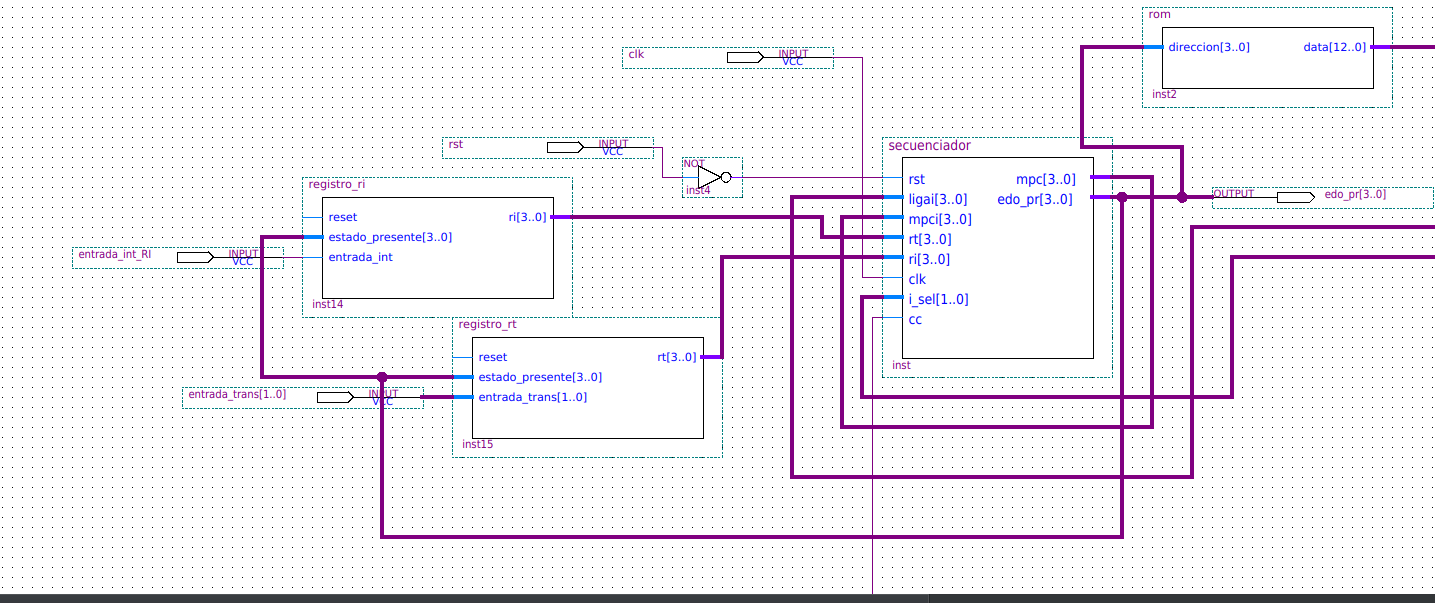
\includegraphics[width=\linewidth]{diagramas_bloques_1.png}
\caption{Interconexión de la ruta de microdirección del secuenciador.}
\label{fig:interconexion-1}
\end{figure}

Por ultimo se tienen dos bloques \texttt{divisor\_datos} y \texttt{mux\_entradas}, el primero se encarga de separar los campos de la microinstrucción, mientras que el segundo selecciona la condición que se va a evaluar, ya sea $X$, $Y$ o \texttt{INT}. Adicionalmente se tiene una compuerta XOR entre el $VF$ y la salida del \texttt{mux\_entradas}, la cual genera la condición final que se va a evaluar en el secuenciador.

\begin{figure}[H]
\centering
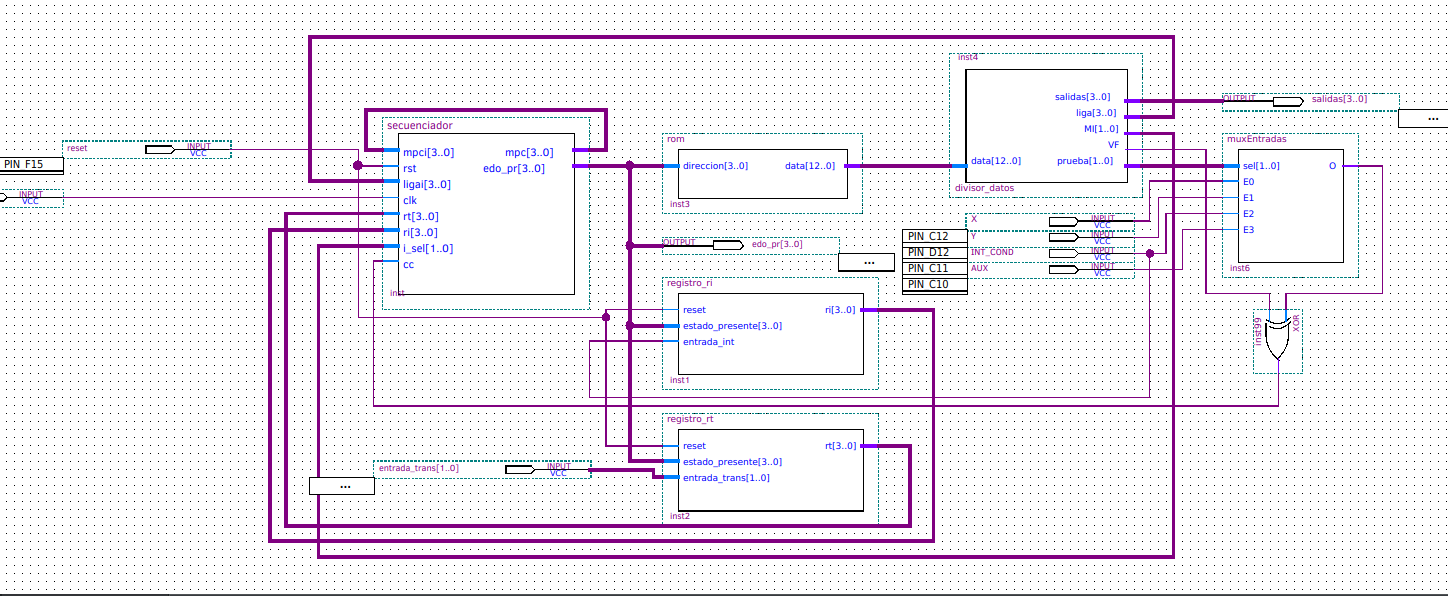
\includegraphics[width=\linewidth]{diagramas_bloques_2.png}
\caption{Interconexión de la memoria ROM, el divisor de datos y la ruta de control.}
\label{fig:interconexion-2}
\end{figure}

\begin{figure}[H]
\centering
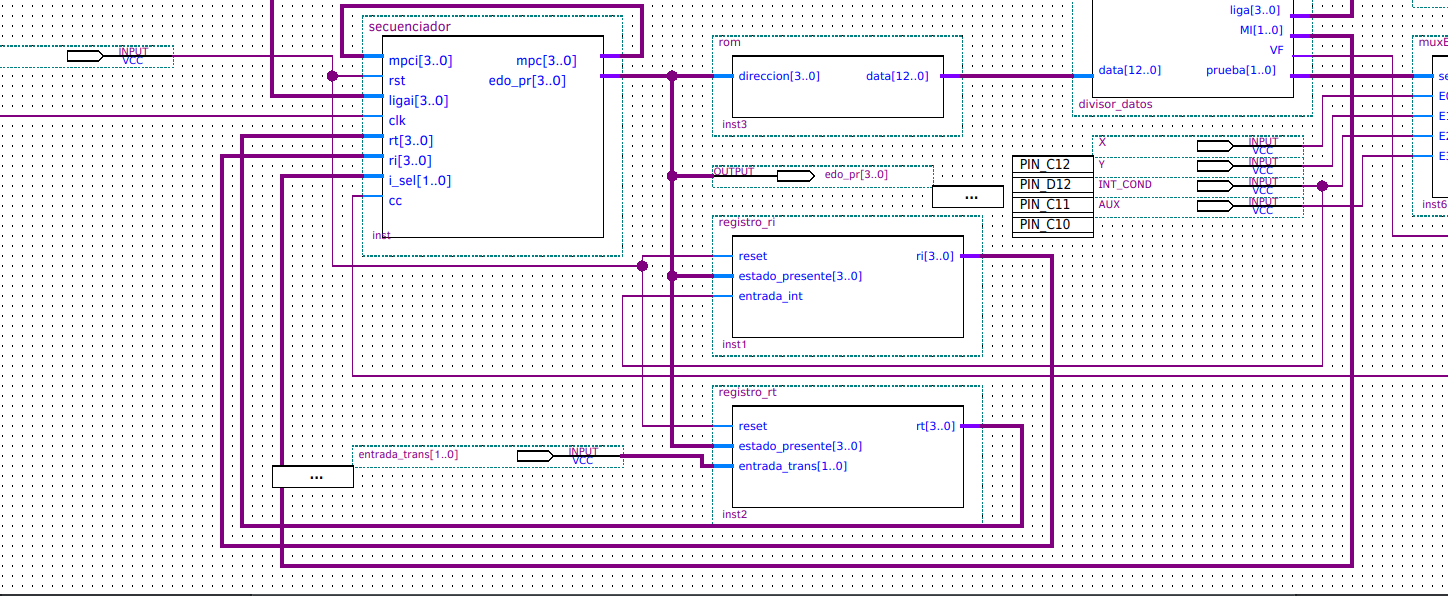
\includegraphics[width=\linewidth]{diagramas_bloques_3.png}
\caption{Diagrama final de bloques del secuenciador microprogramado.}
\label{fig:interconexion-3}
\end{figure}

\subsection{Módulos implementados en VHDL}

\paragraph{Memoria y divisor de campos}: La memoria ROM y el divisor de datos son componentes clave del sistema, \texttt{rom} almacena las dieciséis microinstrucciones de 13 bits. \texttt{divisor\_datos} separa cada palabra en los campos de prueba, inversión, modo, liga y salidas.

\lstinputlisting[style=estiloVHDL,caption={Memoria ROM de 16 palabras por 13 bits.},label={lst:rom}]{code/rom.vhd}

\lstinputlisting[style=estiloVHDL,caption={Divisor de los campos de una microinstrucción.},label={lst:divisor}]{code/divisor_datos.vhd}

\paragraph{Selección de condiciones y direcciones.}: \texttt{muxEntradas} selecciona una de las entradas $X$, $Y$, \texttt{INT} o \texttt{AUX}. \texttt{logica} interpreta el campo $MI$ y determina si se avanza, se usa la liga o se salta a transformación o interrupción. \texttt{incrementador} calcula la siguiente dirección secuencial y \texttt{mux} selecciona entre ella, la liga, \texttt{RT} o \texttt{RI}.

Es importante destacar que para implementar la lógica del registro de interrupción y transformación, se decidió considerarlo como señales de entrada para poder seleccionar que registro se va a utilizar, por otro lado la lógica implementada era por medio de una sentencia condicional evaluar la señal de entrada correspondiente a cada registro, de forma que se evalúa si el estado presente es igual a los estados donde hay un salto a transformación o interrupción, de ser así se selecciona la señal de entrada correspondiente, de lo contrario continua el recorrido normal de microinstrucciones.

\lstinputlisting[style=estiloVHDL,caption={Multiplexor de entradas para la condición de control.},label={lst:mux-entradas}]{code/muxEntradas.vhd}

\lstinputlisting[style=estiloVHDL,caption={Lógica que decodifica el tipo de microinstrucción.},label={lst:logica}]{code/logica.vhd}

\lstinputlisting[style=estiloVHDL,caption={Incrementador de la microdirección.},label={lst:incrementador}]{code/incrementador.vhd}

\lstinputlisting[style=estiloVHDL,caption={Multiplexor de la siguiente microdirección.},label={lst:mux}]{code/mux.vhd}

\paragraph{Registros y avance por botón.} \texttt{registro\_mpc} conserva la microdirección y la actualiza en cada flanco ascendente, con reinicio a cero. \texttt{registro\_rt} y \texttt{registro\_ri} generan las direcciones de transformación e interrupción según el estado y sus entradas. \texttt{clk\_buttom} es un divisor de frecuencia que genera un pulso de avance por cada pulsación del botón.

\lstinputlisting[style=estiloVHDL,caption={Registro del contador de microprograma.},label={lst:mpc}]{code/registro_mpc.vhd}

\lstinputlisting[style=estiloVHDL,caption={Registro de transformación.},label={lst:rt}]{code/registro_rt.vhd}

\lstinputlisting[style=estiloVHDL,caption={Registro de interrupción.},label={lst:ri}]{code/registro_ri.vhd}

\lstinputlisting[style=estiloVHDL,caption={Generador de un avance por pulsación.},label={lst:paso}]{code/clk_buttom.vhd}

\section{Simulación}

La simulación se realizó aplicando una señal de reloj periódica, manteniendo
\texttt{reset=1}, se fueron modificando las entradas $X$, $Y$,
\texttt{INT}, \texttt{AUX} y \texttt{entrada\_trans}. En las formas de onda se
observan la dirección presente \texttt{edo\_pr}, las salidas de la ROM
\texttt{salidas}, el selector de prueba, las entradas de la carta ASM, el reloj y
el reinicio. La dirección sólo cambia en los flancos ascendentes del reloj, por lo que \texttt{edo\_pr} permanece estable durante el intervalo
correspondiente a una microinstrucción.

En la Figura[\ref{fig:sim-1}] se puede observar el recorrido inicial del secuenciador.
La dirección parte de \texttt{0000}, donde la ROM entrega las salidas
\texttt{1100} y el campo $MI=\texttt{00}$ selecciona el avance secuencial hacia
\texttt{0001}. En esa dirección se activa el salto de transformación
($MI=\texttt{10}$), por lo que la siguiente dirección depende de
\texttt{entrada\_trans}. En la forma de onda se pueden apreciar varios recorridos posibles, como
$\texttt{0000}\rightarrow\texttt{0001}\rightarrow\texttt{0010}$ y
$\texttt{0000}\rightarrow\texttt{0001}\rightarrow\texttt{1000}$.
Estos recorridos corresponden a diferentes valores de la entrada de
transformación: desde $E_1$ se puede dirigir el secuenciador a $E_2$,
$E_8$ o $E_{13}$, dependiendo de la señal de entrada. Posteriormente, la microinstrucción de $E_2$ utiliza la prueba $X$ y
selecciona la liga o el avance según el resultado de la condición.

\begin{figure}[H]
\centering
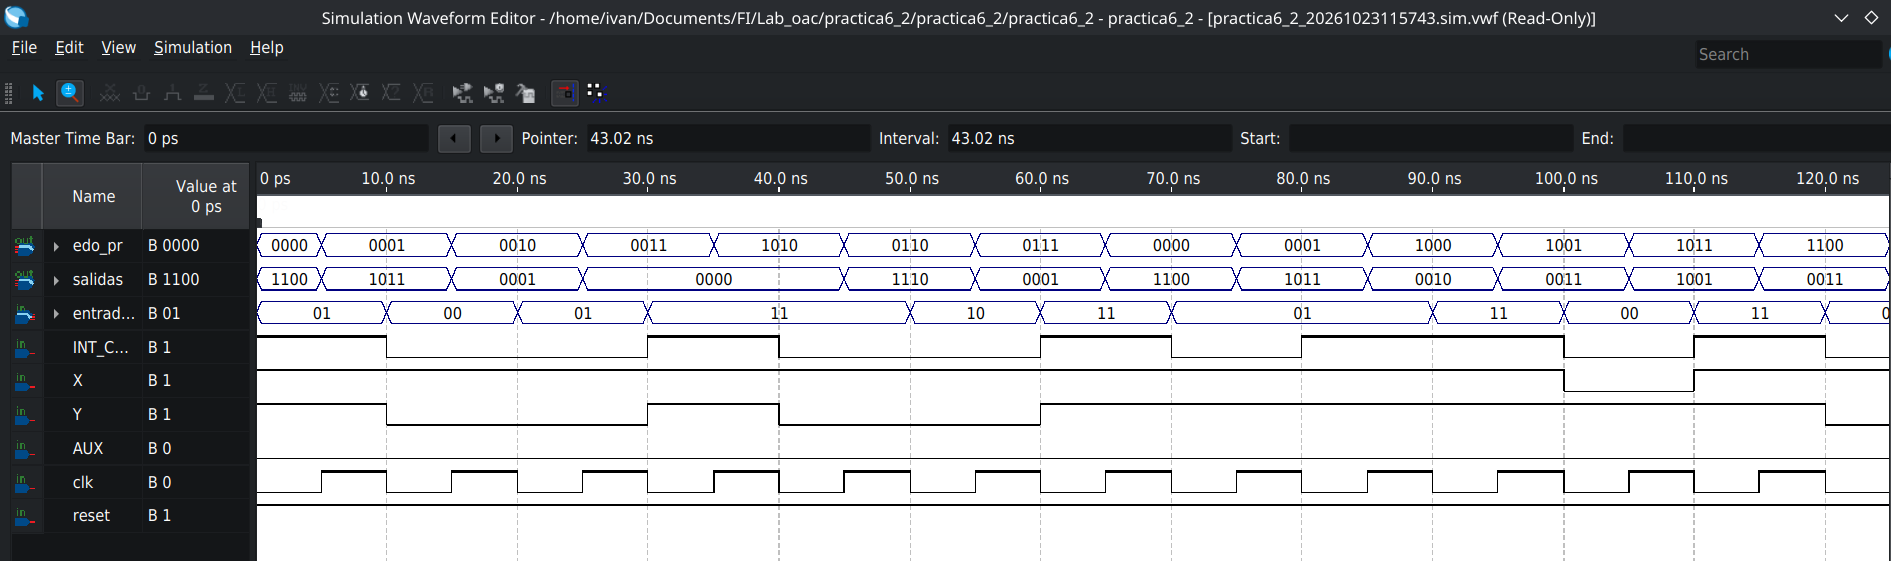
\includegraphics[width=\linewidth]{simulacion_1.png}
\caption{Recorrido inicial de las microdirecciones, salidas de la ROM y entradas de control.}
\label{fig:sim-1}
\end{figure}

La Figura [\ref{fig:sim-2}] muestra una secuencia que inicia en
\texttt{0011}, correspondiente a $E_3$. En este estado la microinstrucción
utiliza $MI=\texttt{11}$, de modo que la dirección se obtiene del registro
\texttt{RI} y depende de \texttt{INT}. Cuando \texttt{INT=0}, el registro
\texttt{RI} produce \texttt{0100}, y el recorrido continúa por
\texttt{0101} hasta regresar a \texttt{0000}. También se observa el recorrido
$\texttt{0001}\rightarrow\texttt{1000}\rightarrow\texttt{1001}$, donde la
primera transición corresponde a una transformación y, en $E_9$, el campo
\texttt{Prueba} selecciona $Y$. Según el valor de $Y$, el secuenciador avanza
a $E_{10}$ o carga la liga de la microinstrucción.

\begin{figure}[H]
\centering
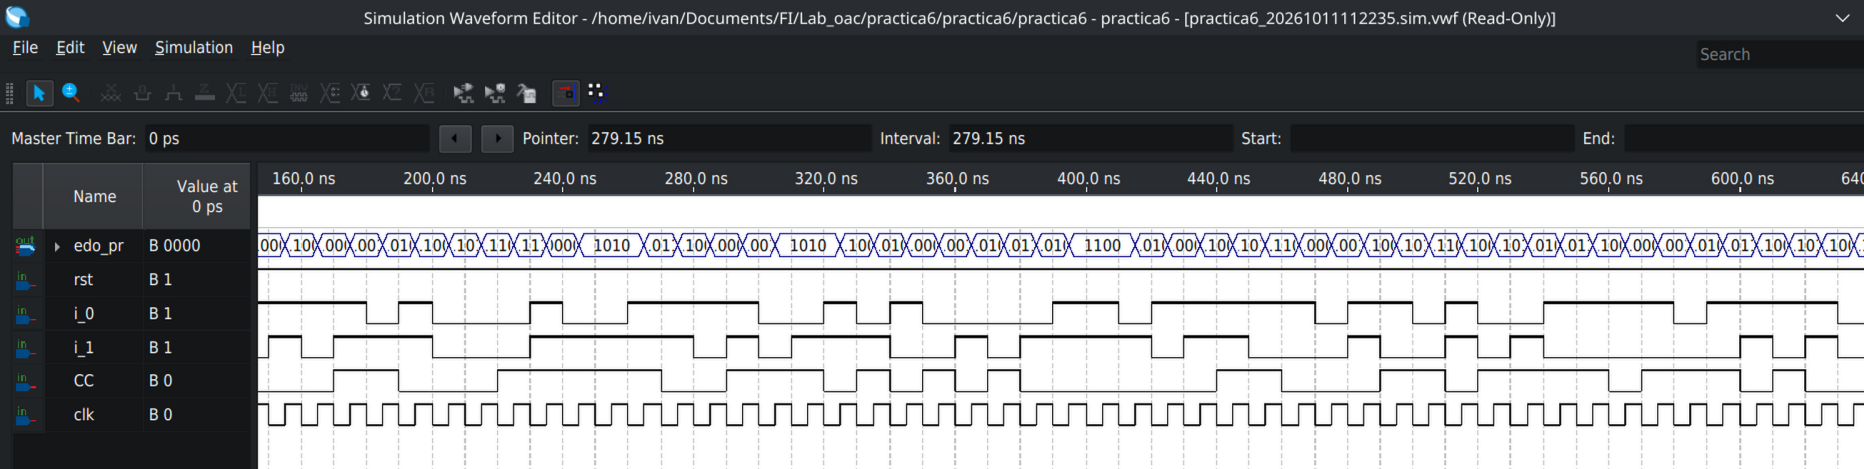
\includegraphics[width=\linewidth]{simulacion_2.png}
\caption{Recorridos con prueba de $Y$ y salto por interrupción desde $E_3$.}
\label{fig:sim-2}
\end{figure}

En la Figura [\ref{fig:sim-3}] se analiza la otra ruta de transformación e
interrupción. La cual inicia desde \texttt{1011} ($E_{11}$), el registr de transformación \texttt{RT} conduce
la secuencia a $E_{12}$ o a $E_7$ según \texttt{entrada\_trans}. Cuando se
selecciona $E_{12}$, la liga \texttt{1110} lleva a $E_{14}$ y la liga de
$E_{14}$ devuelve el control a $E_{11}$. En esta misma parte se observa el
salto por interrupción desde $E_{13}$, cuando \texttt{INT=0} conduce a
\texttt{1110}, mientras que \texttt{INT=1} conduce a \texttt{0001}, de
acuerdo con la tabla de microprogramación. Las señales \texttt{salidas}
adoptan los valores almacenados en la ROM para cada dirección.

\begin{figure}[H]
\centering
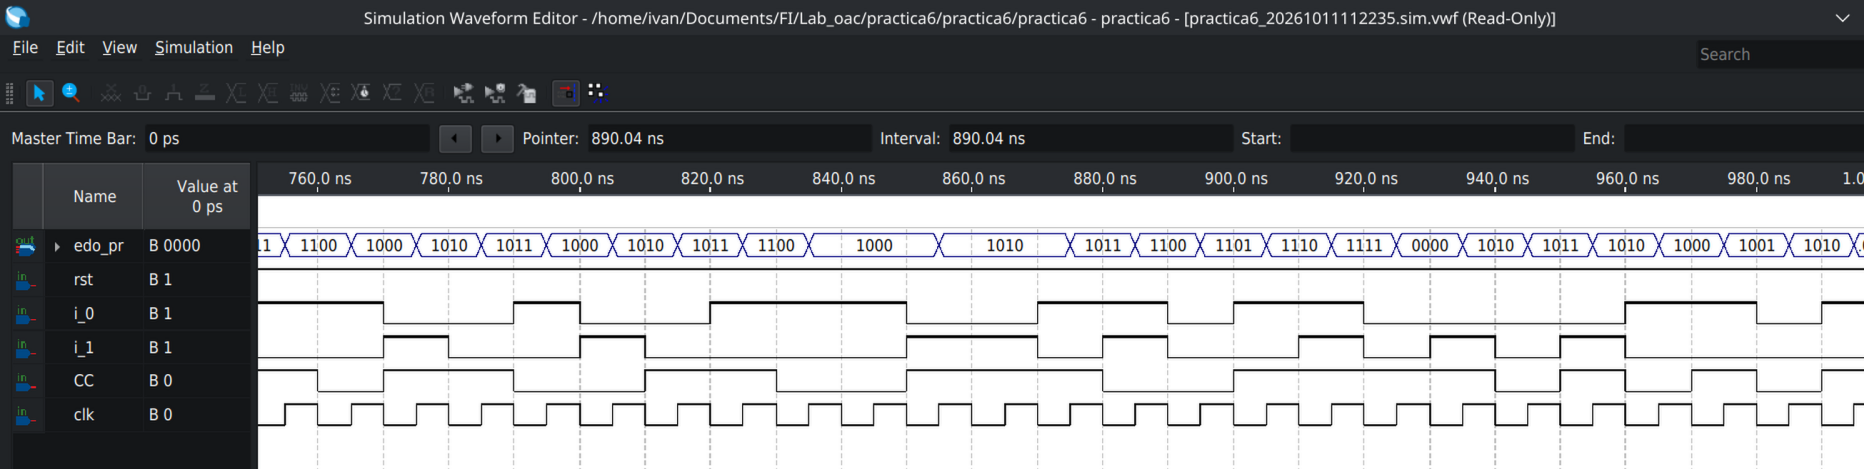
\includegraphics[width=\linewidth]{simulacion_3.png}
\caption{Recorridos de transformación e interrupción en la rama de $E_{11}$ a $E_{14}$.}
\label{fig:sim-3}
\end{figure}

\section{Resultados en la tarjeta FPGA}

Al implementar el circuito en la FPGA DE10-Lite, se observan el estado presente mediante los LEDs. Los LEDs de la izquierda muestran las salidas de la carta ASM, mientras que los LEDs de la derecha indican el estado presente, a su vez cada que se presiona el botón, el secuenciador avanza un estado, permitiendo verificar la correspondencia entre la carta ASM y la implementación física.

\begin{figure}[H]
\centering
\begin{subfigure}[b]{0.19\linewidth}\centering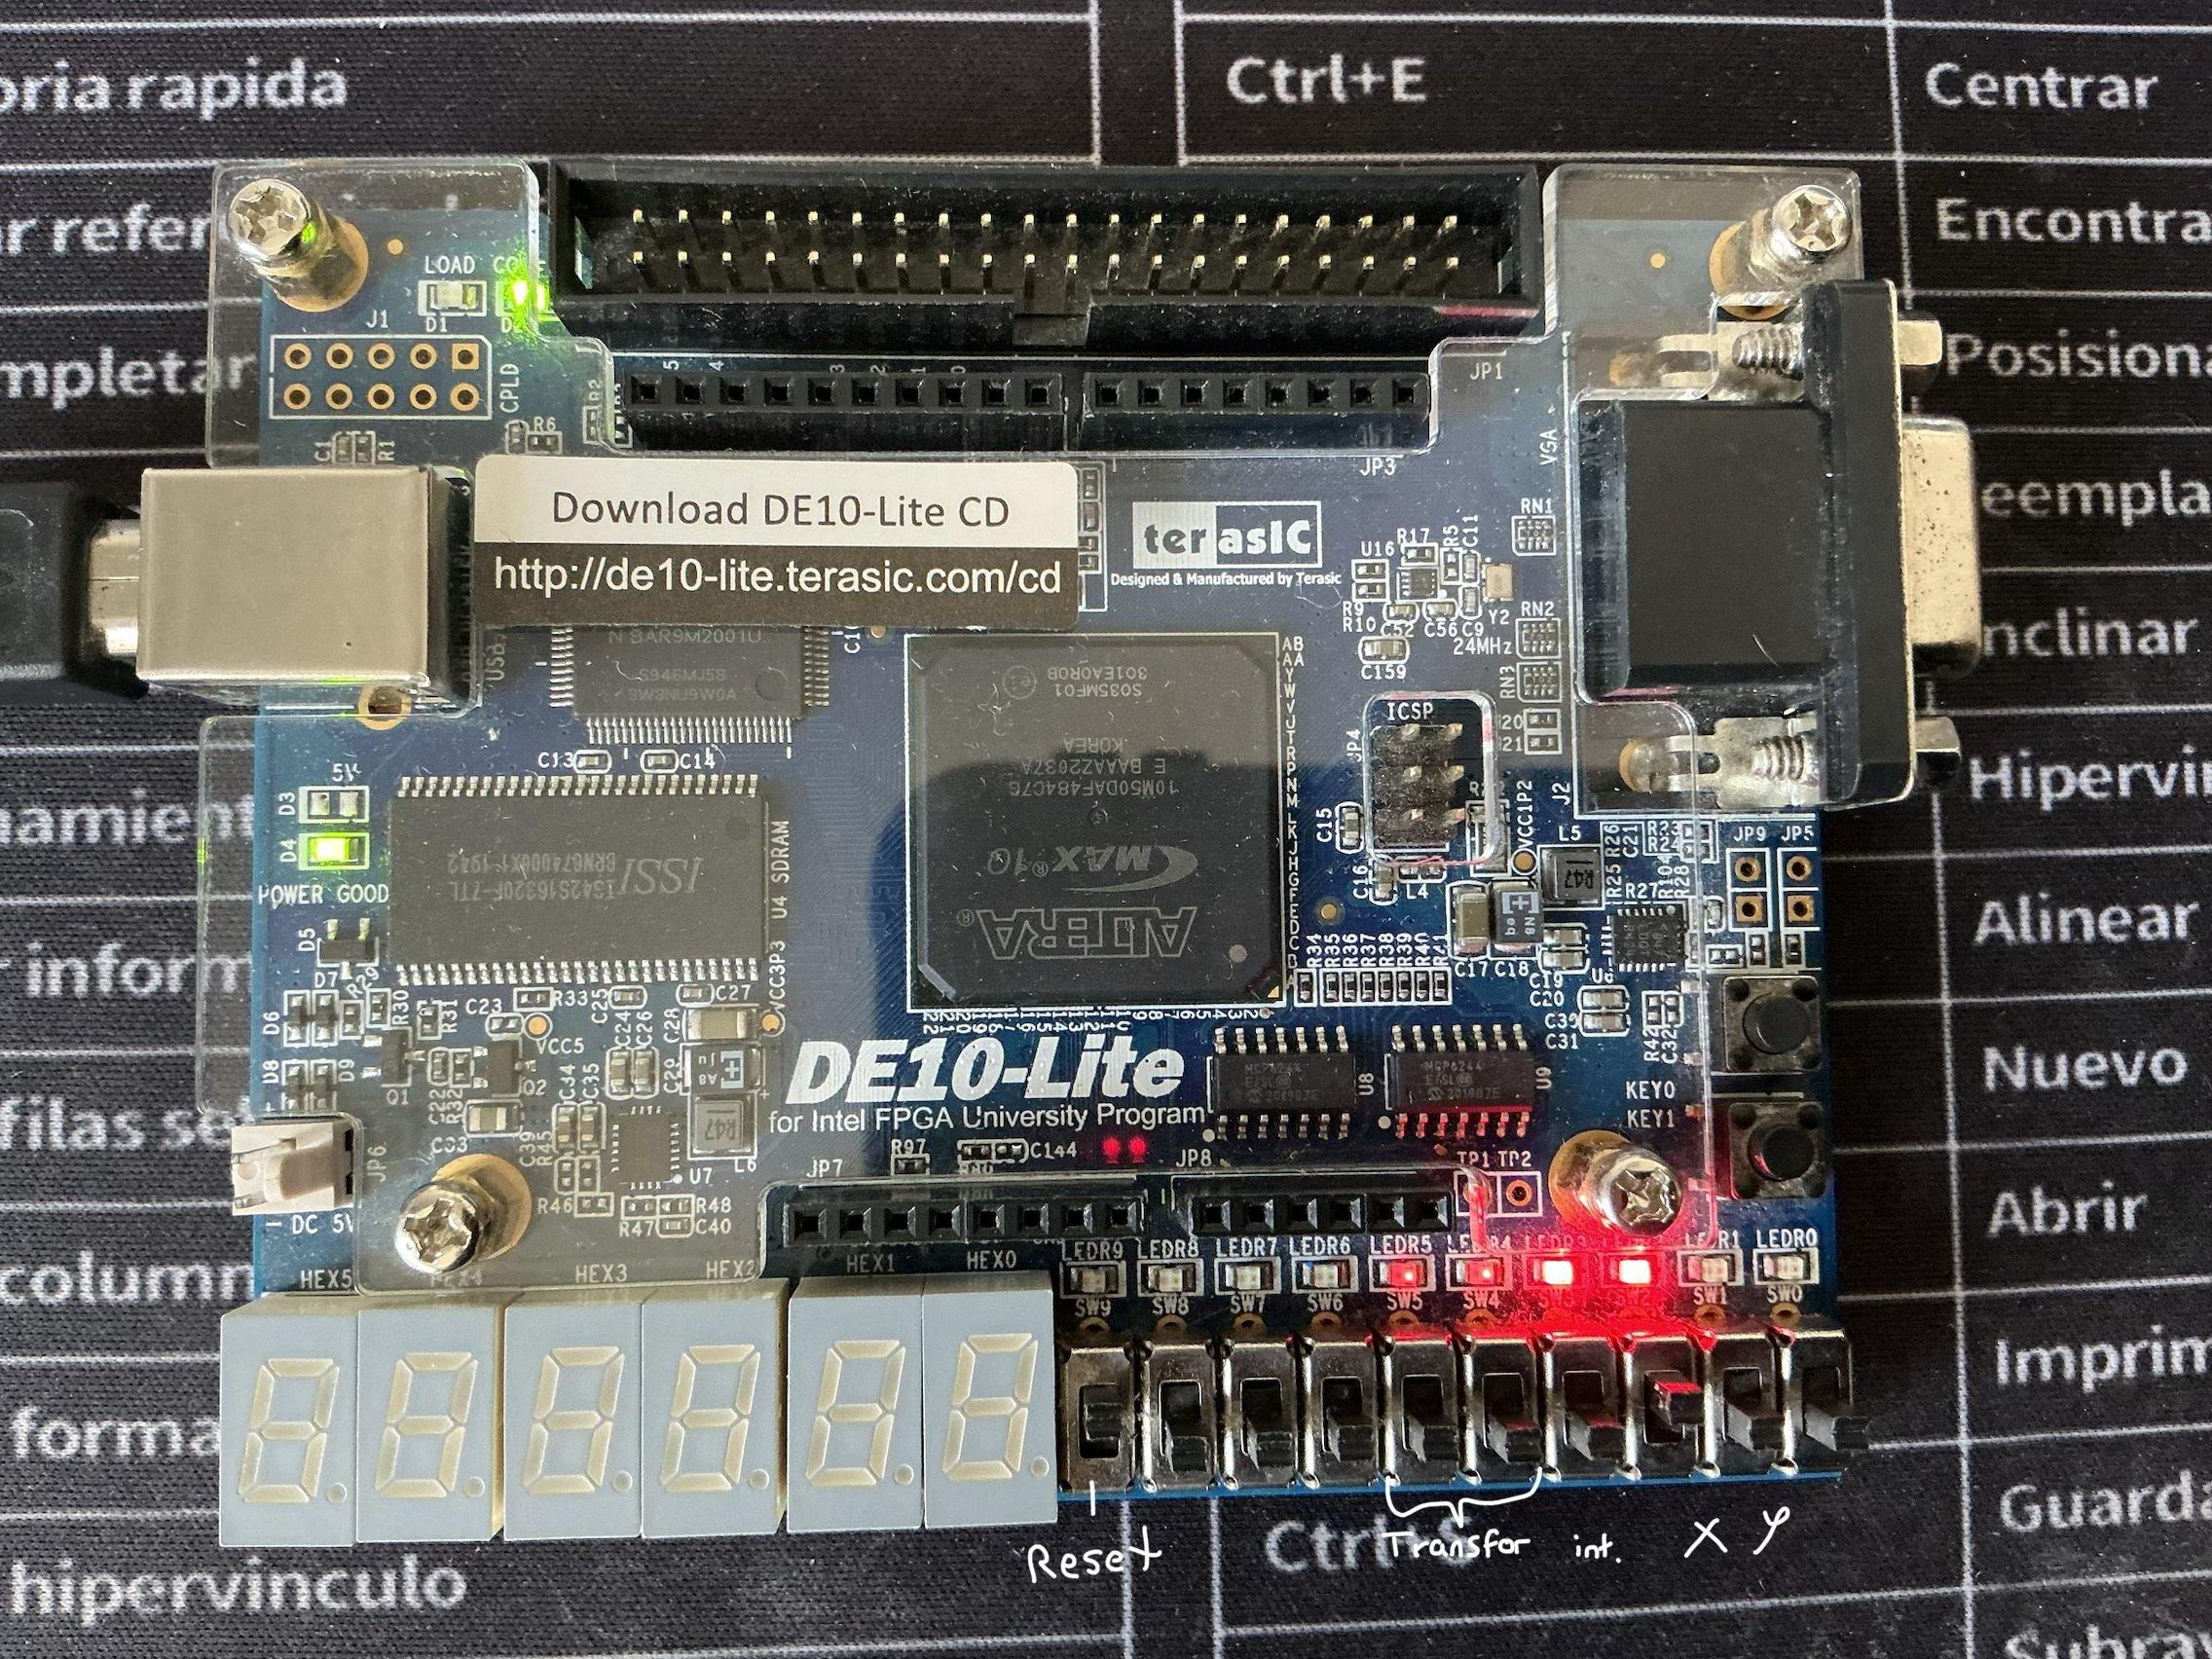
\includegraphics[width=\linewidth]{est0.jpg}\caption{$E_0$}\end{subfigure}\hfill
\begin{subfigure}[b]{0.19\linewidth}\centering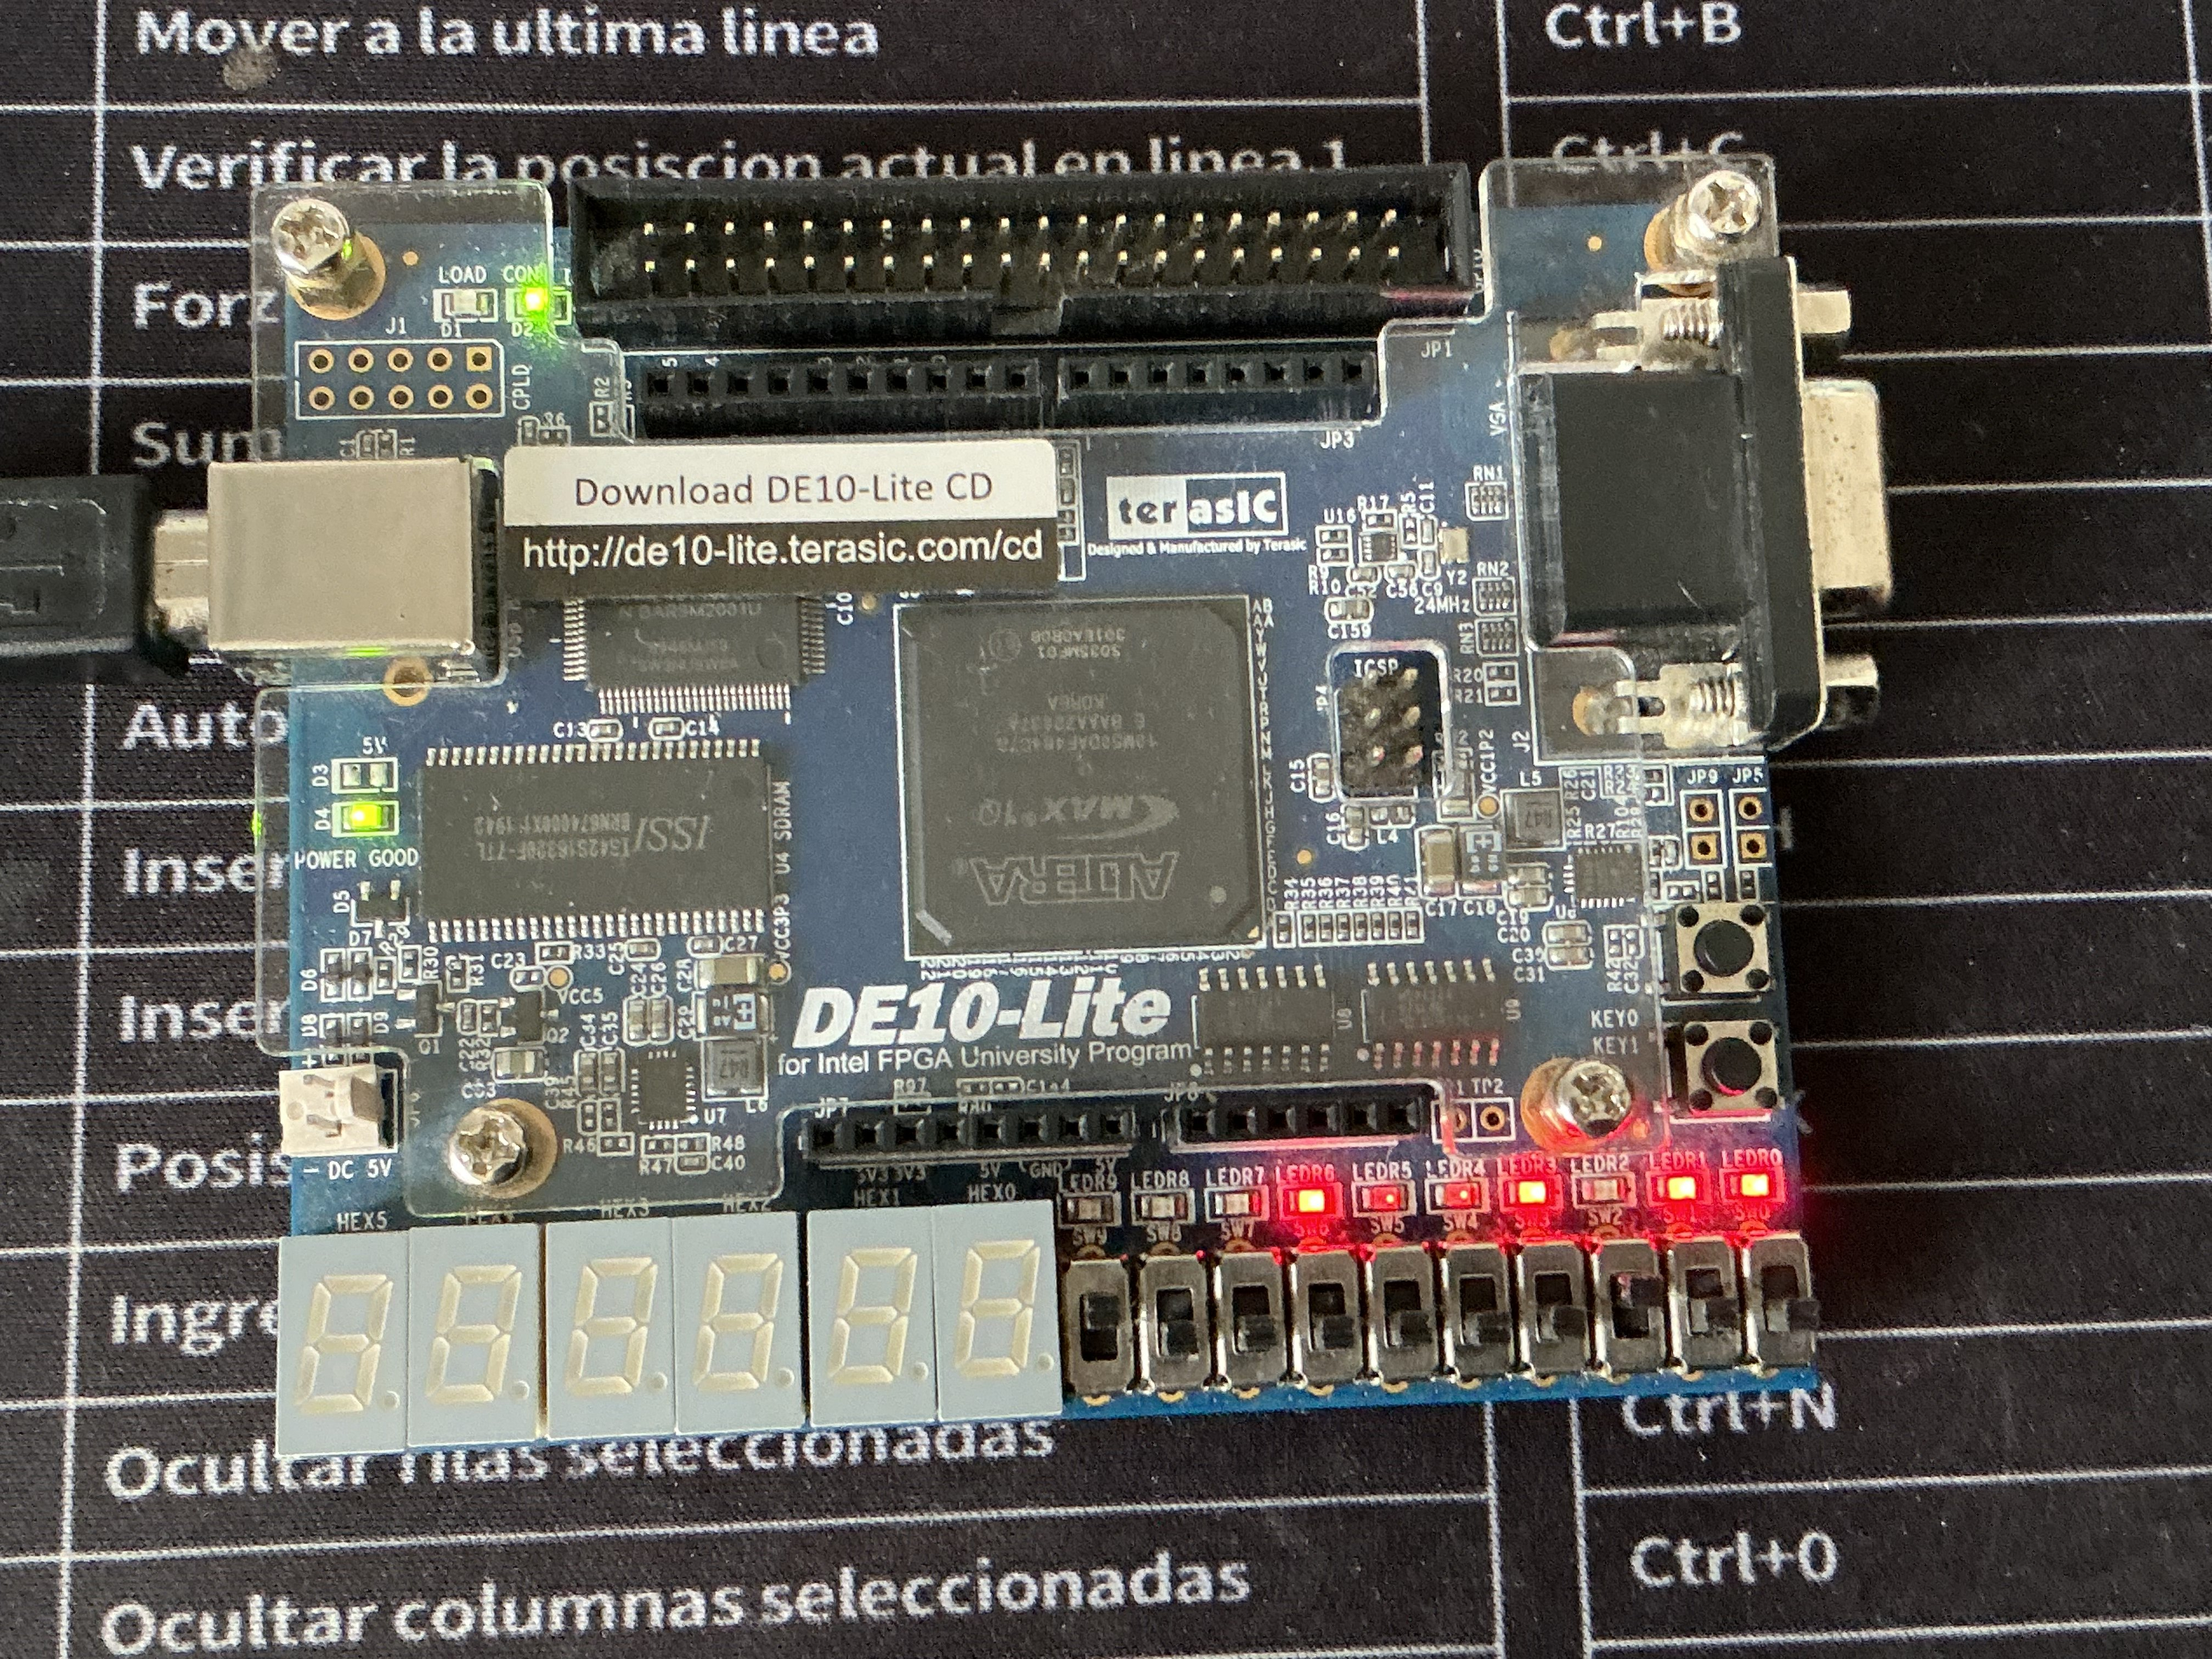
\includegraphics[width=\linewidth]{est01.jpg}\caption{$E_1$}\end{subfigure}\hfill
\begin{subfigure}[b]{0.19\linewidth}\centering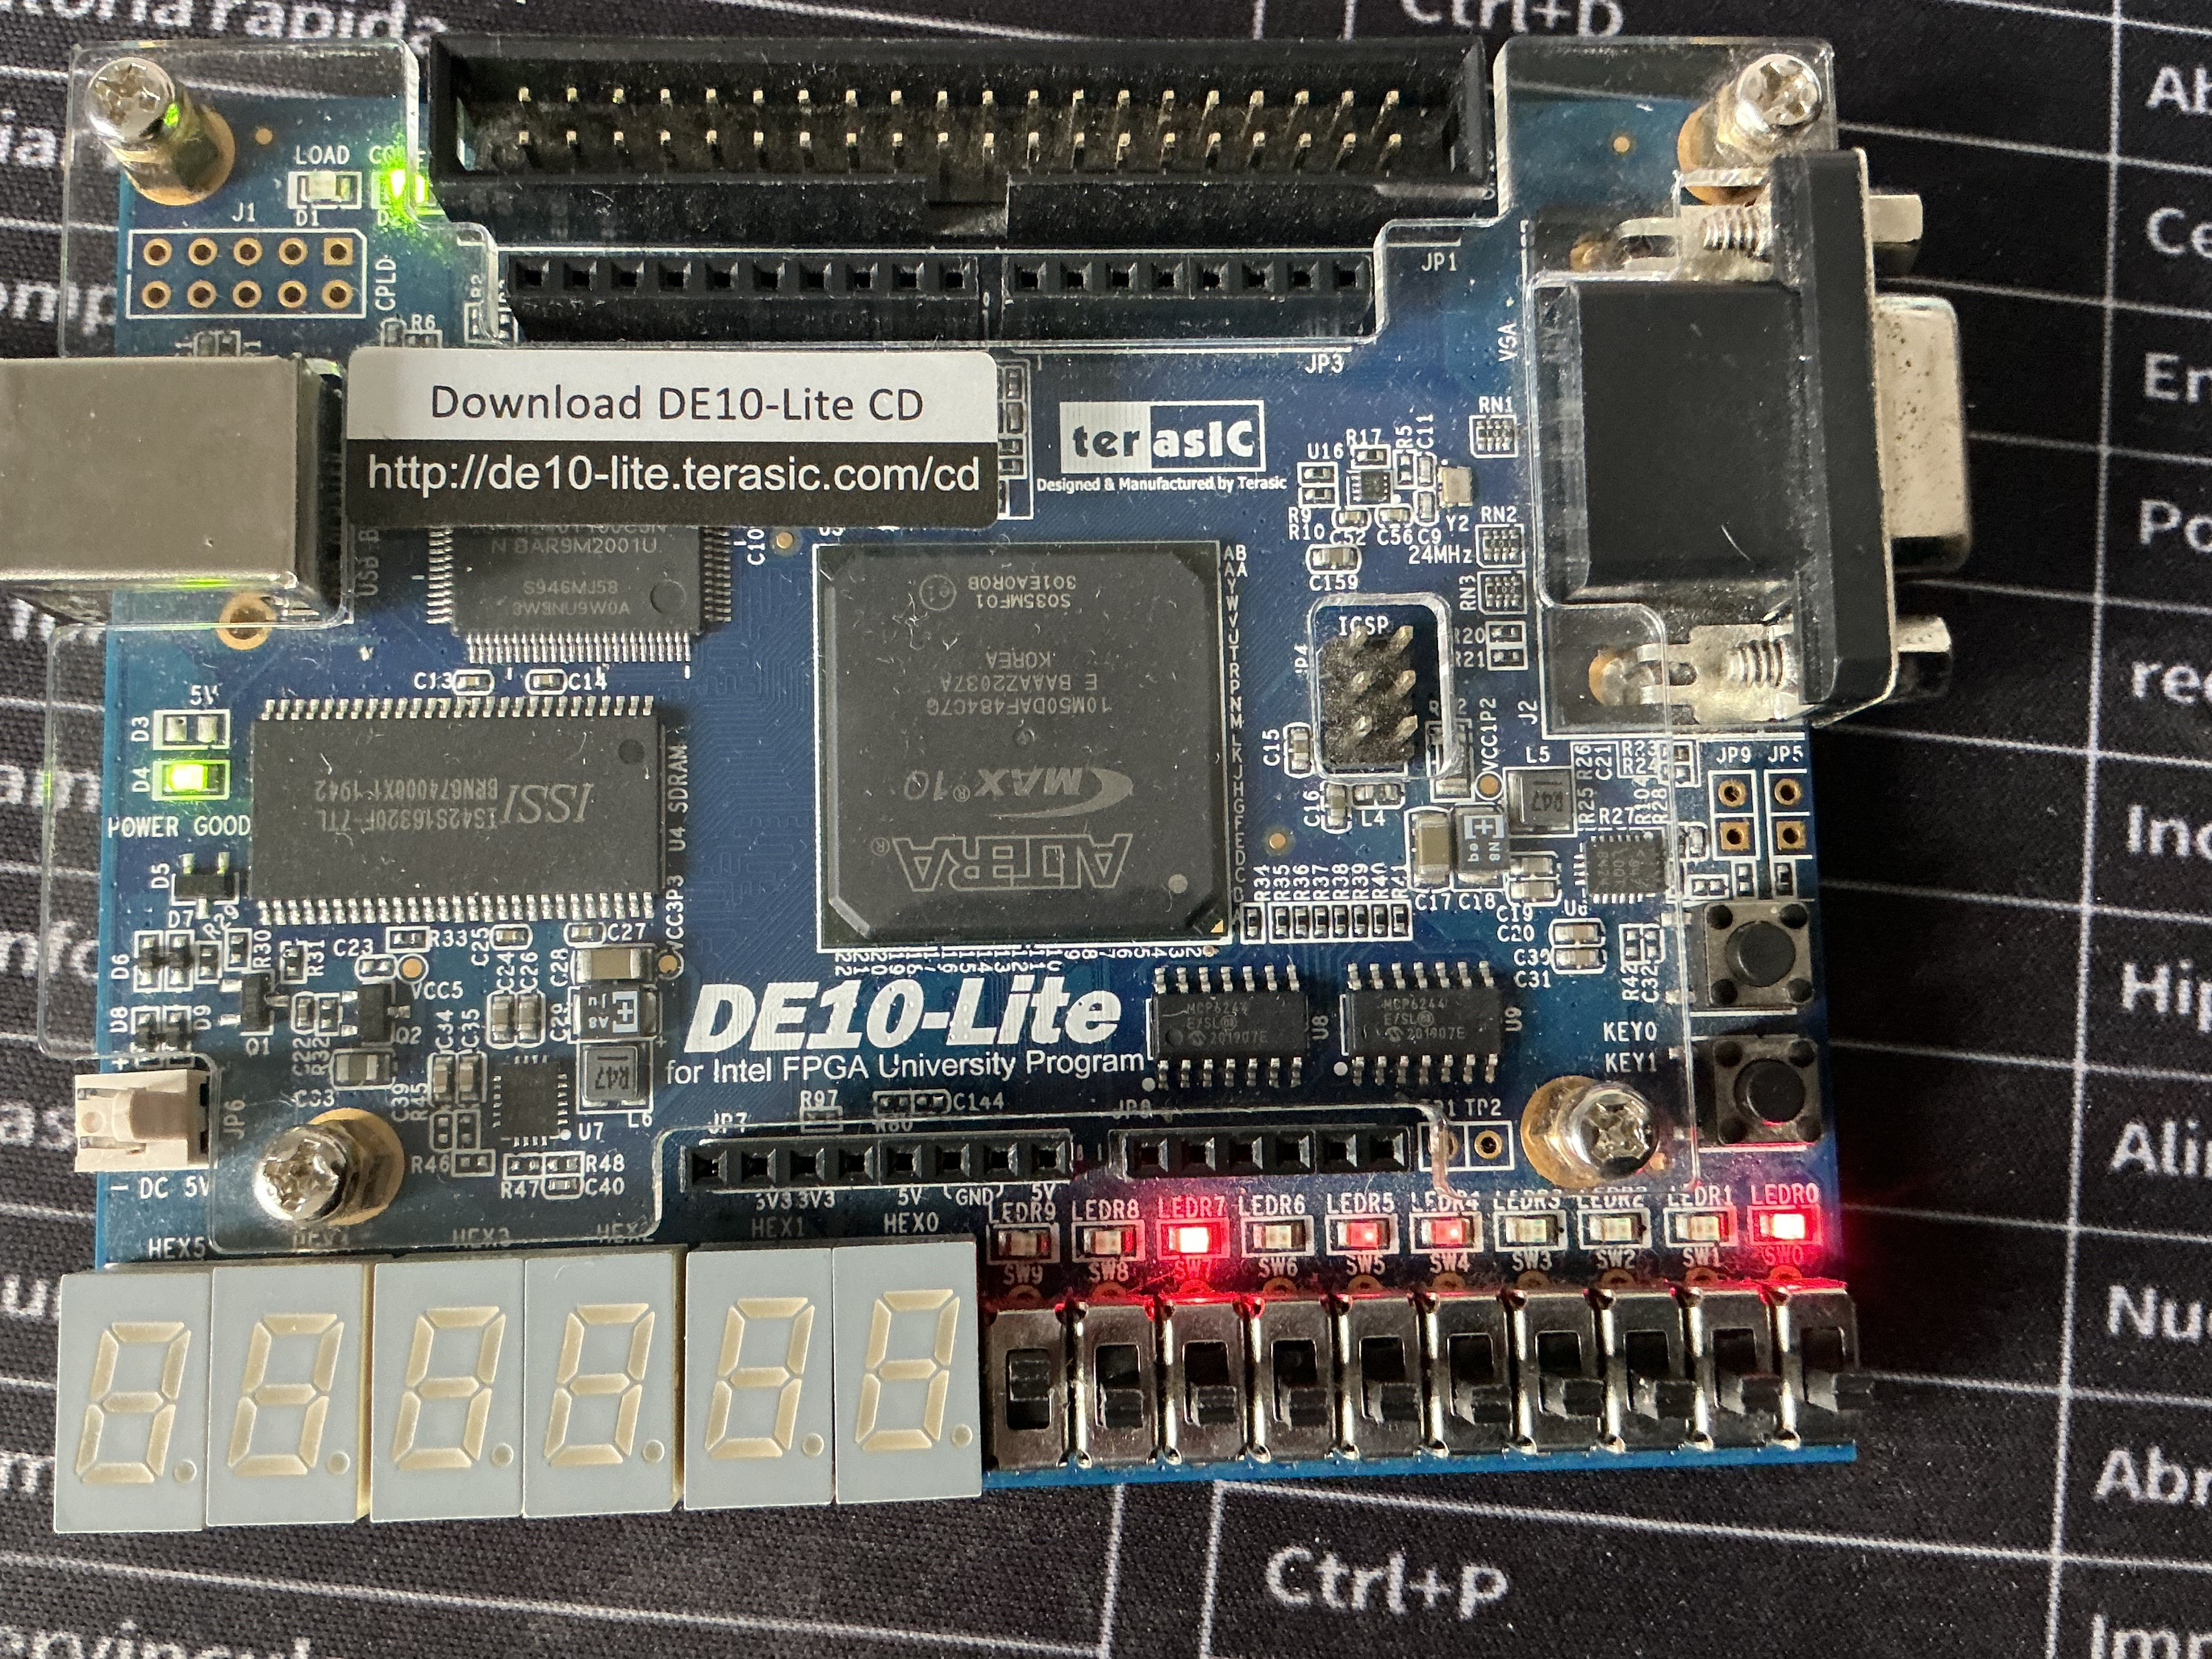
\includegraphics[width=\linewidth]{est02.jpg}\caption{$E_2$}\end{subfigure}\hfill
\begin{subfigure}[b]{0.19\linewidth}\centering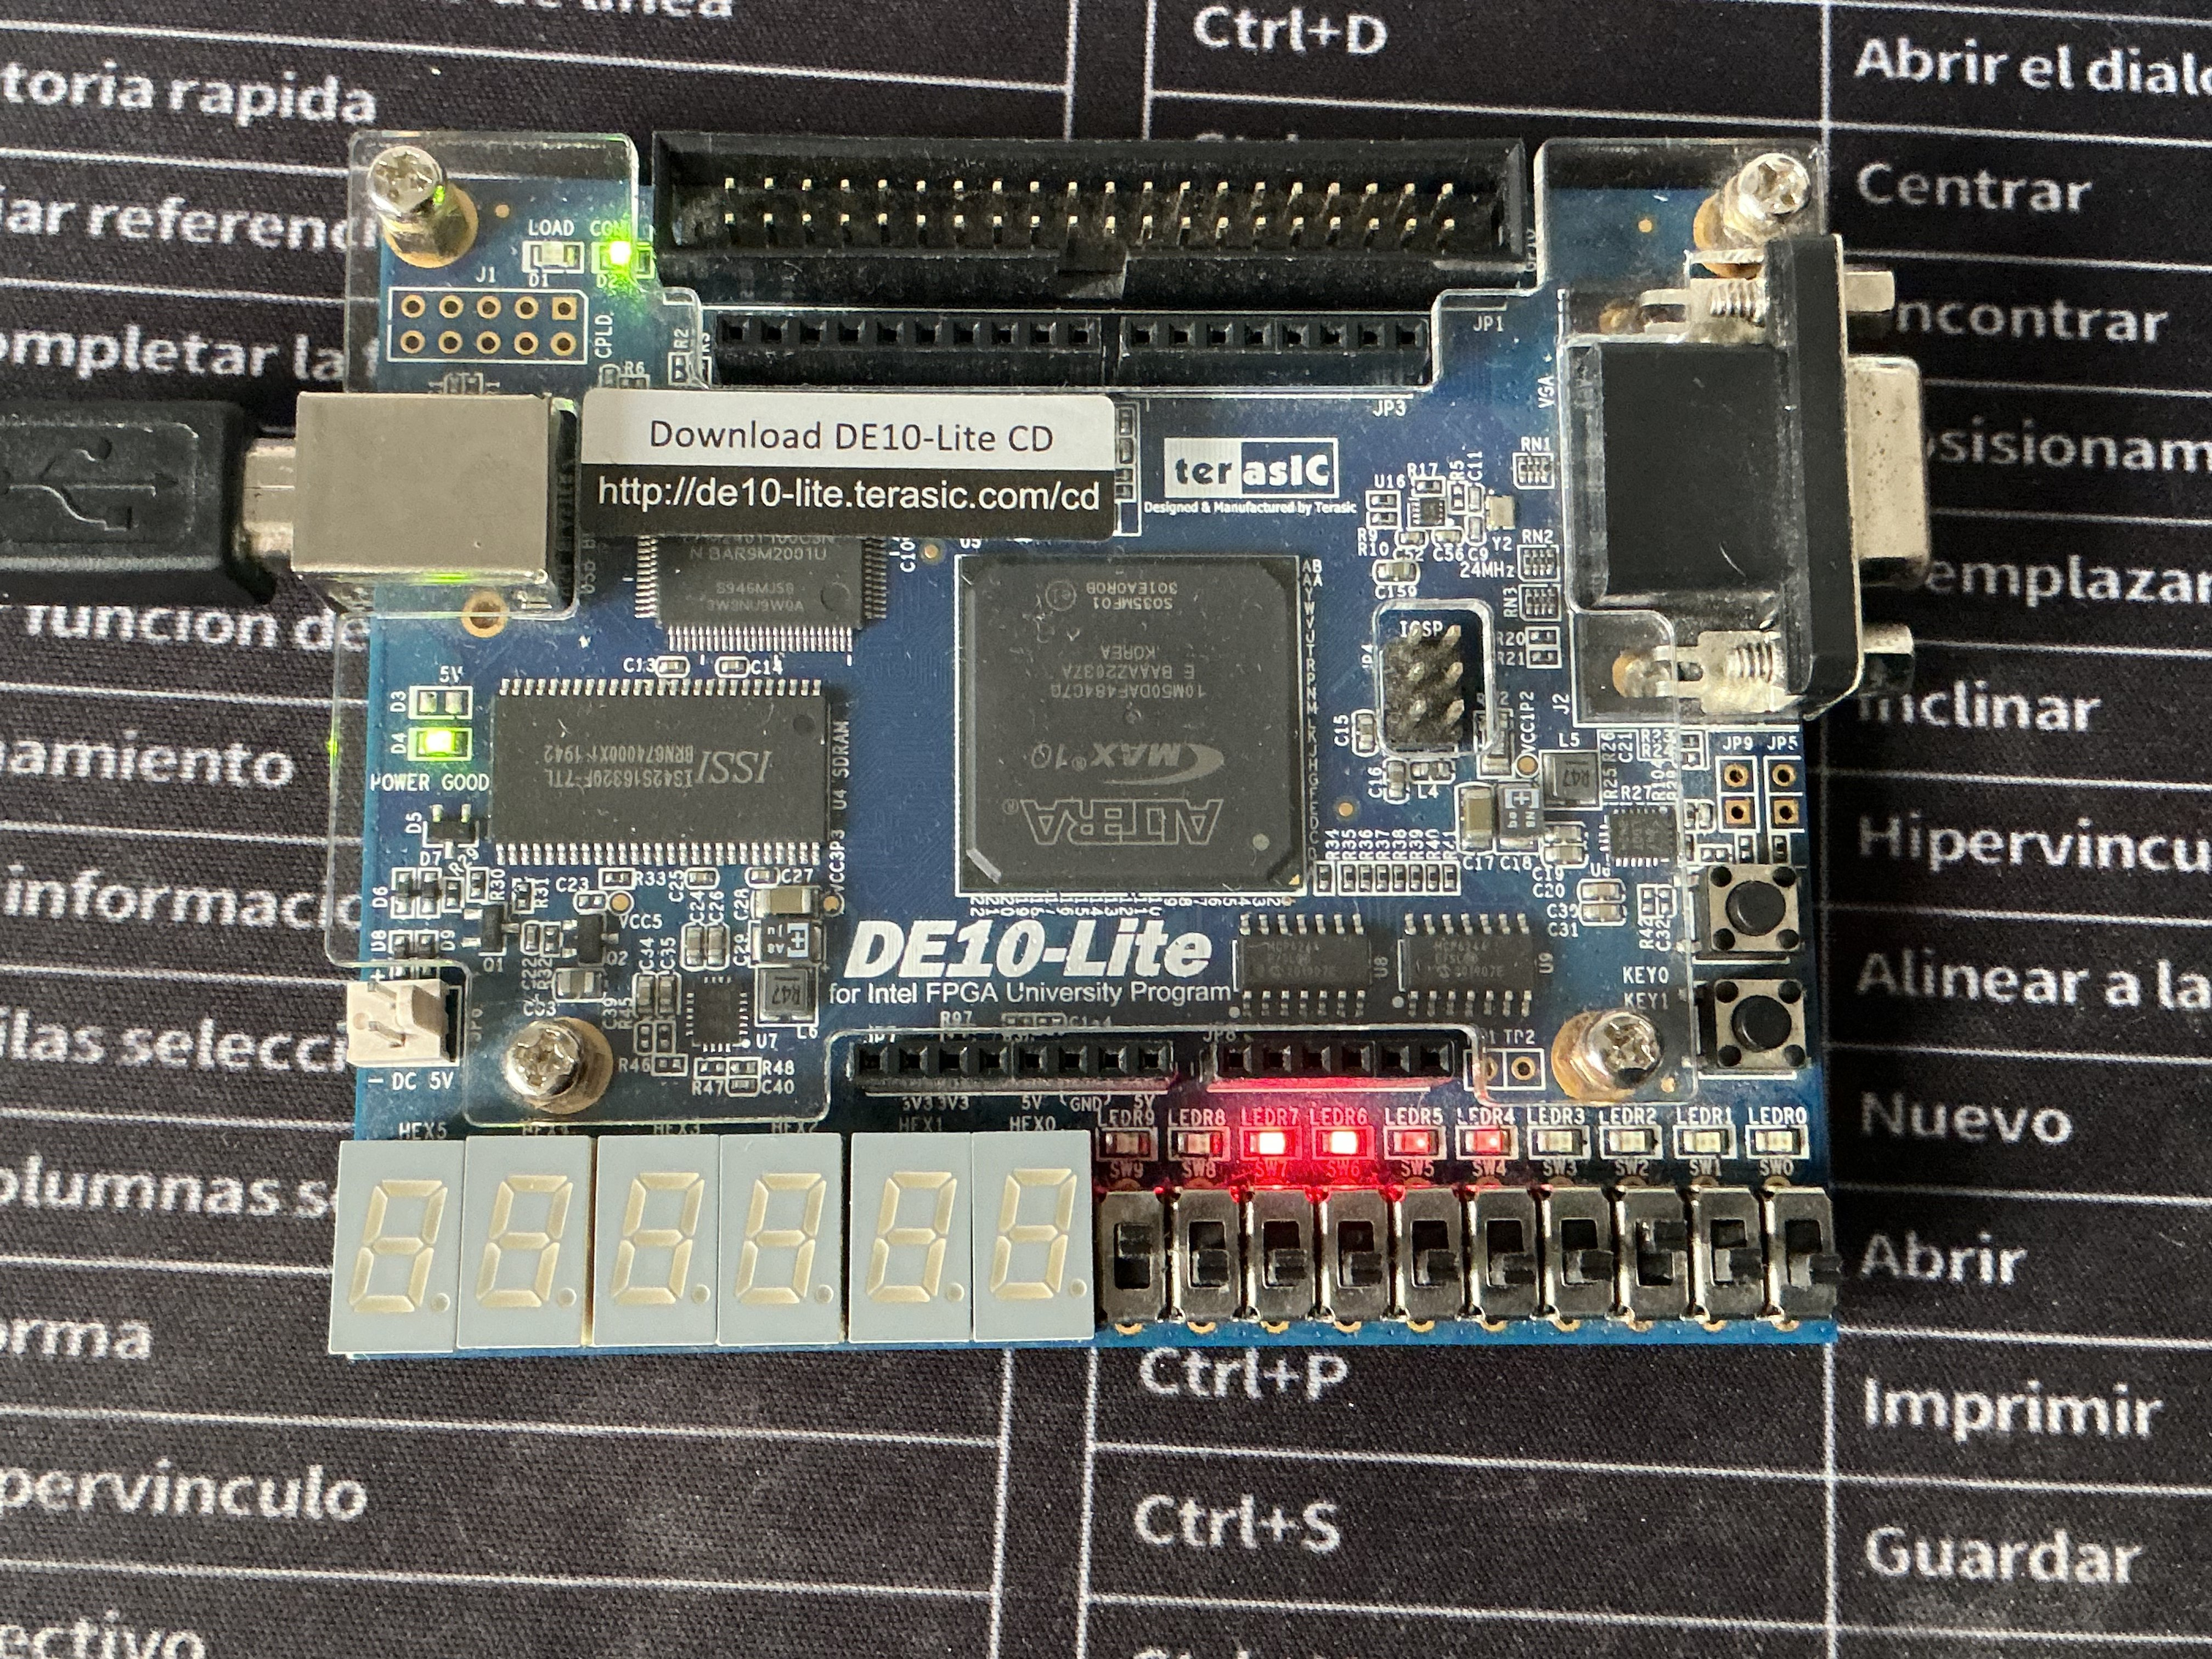
\includegraphics[width=\linewidth]{est03.jpg}\caption{$E_3$}\end{subfigure}\hfill
\begin{subfigure}[b]{0.19\linewidth}\centering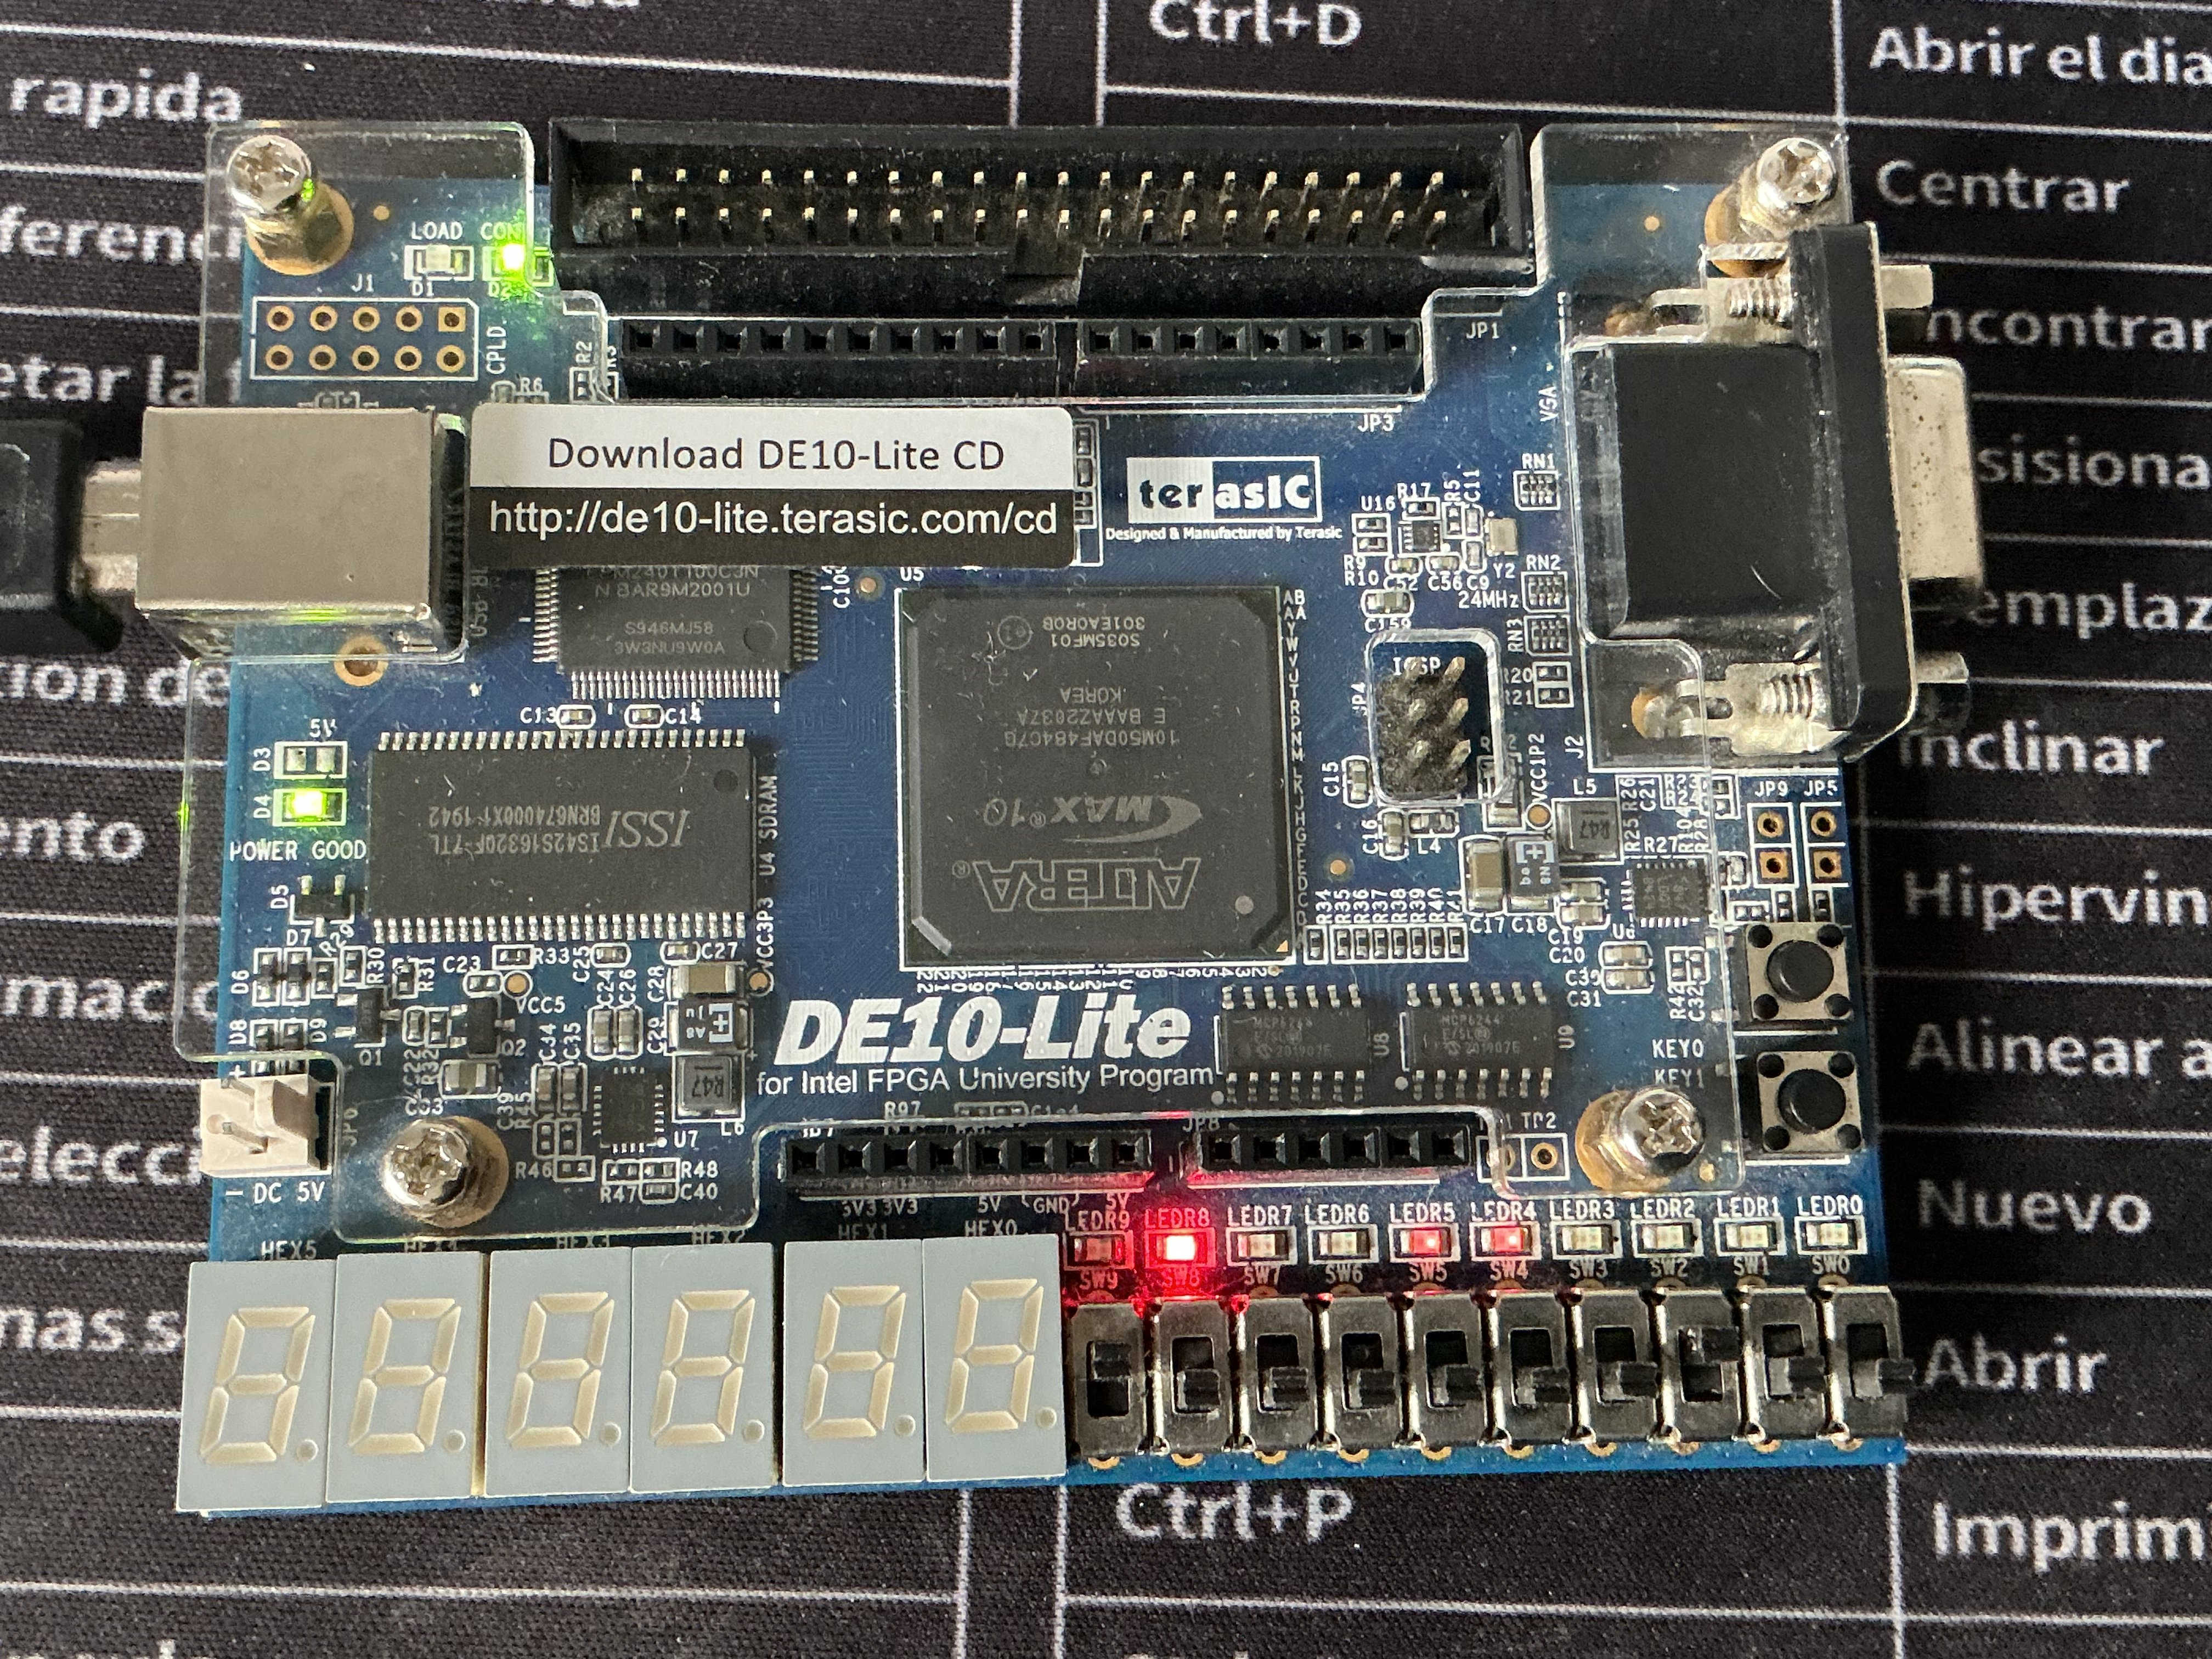
\includegraphics[width=\linewidth]{est04.jpg}\caption{$E_4$}\end{subfigure}
\caption{Estados iniciales observados en la tarjeta DE10-Lite.}
\label{fig:fpga-0-4}
\end{figure}

\begin{figure}[H]
\centering
\begin{subfigure}[b]{0.19\linewidth}\centering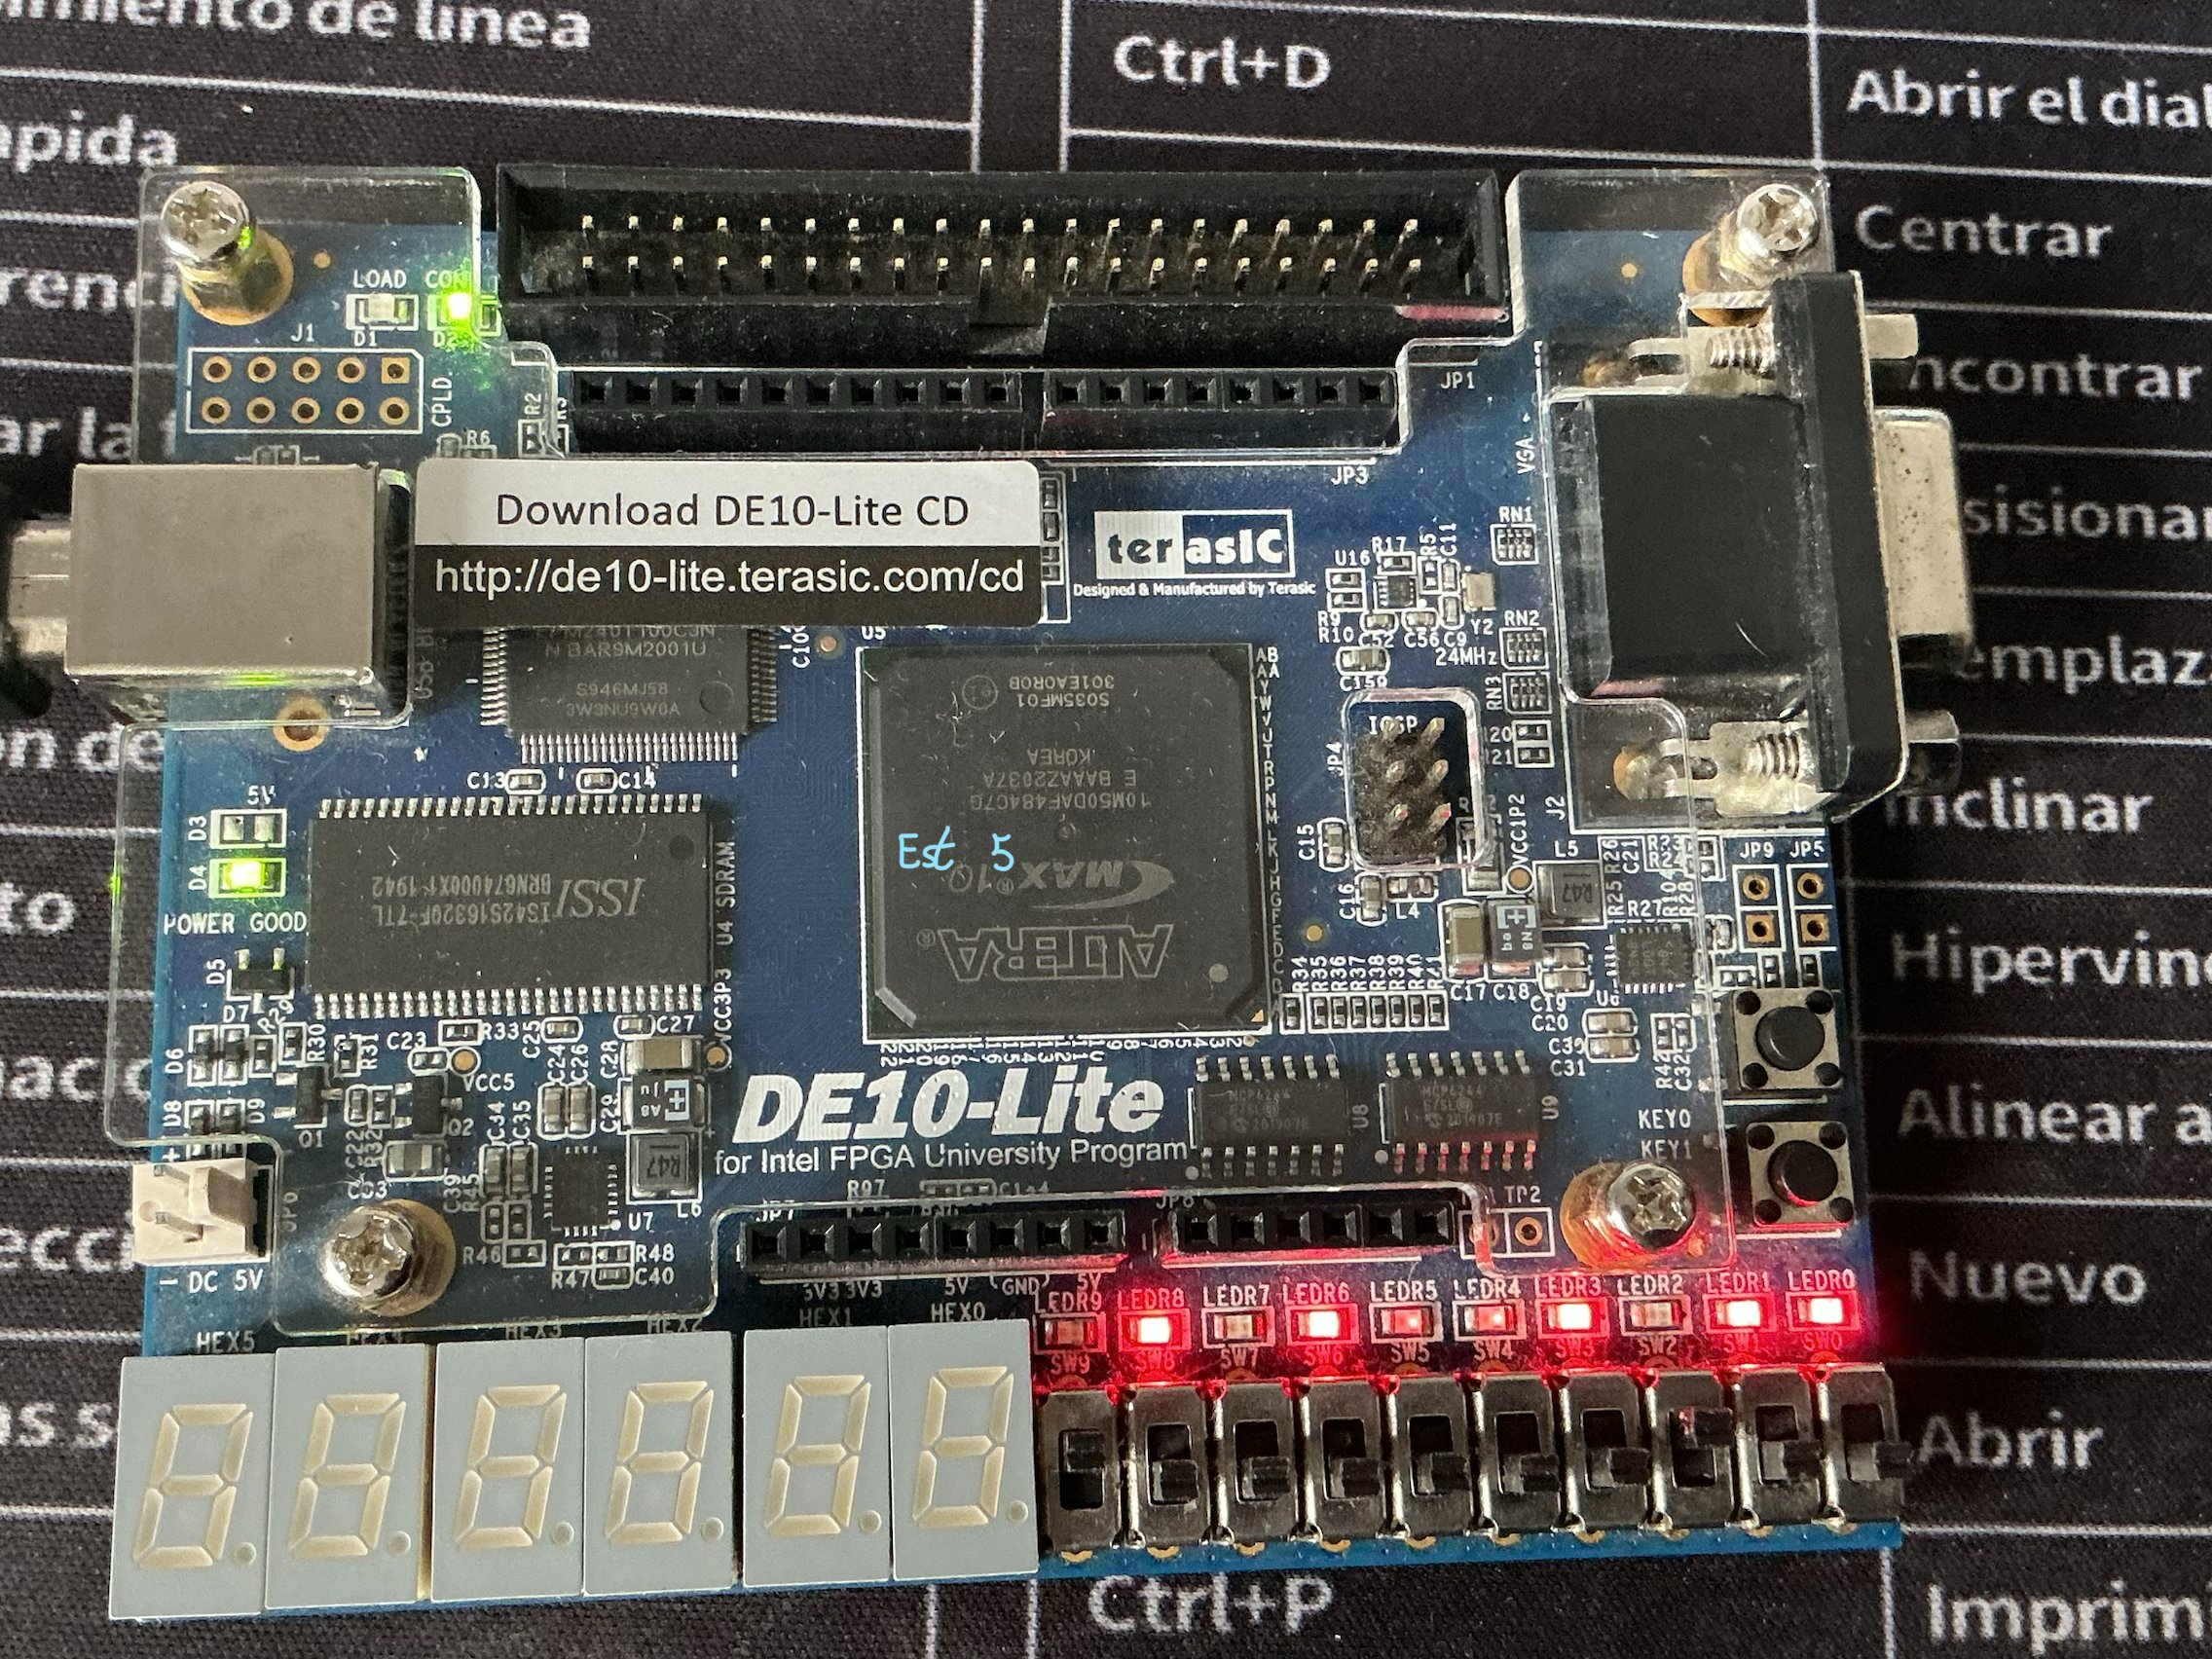
\includegraphics[width=\linewidth]{est05.jpg}\caption{$E_5$}\end{subfigure}\hfill
\begin{subfigure}[b]{0.19\linewidth}\centering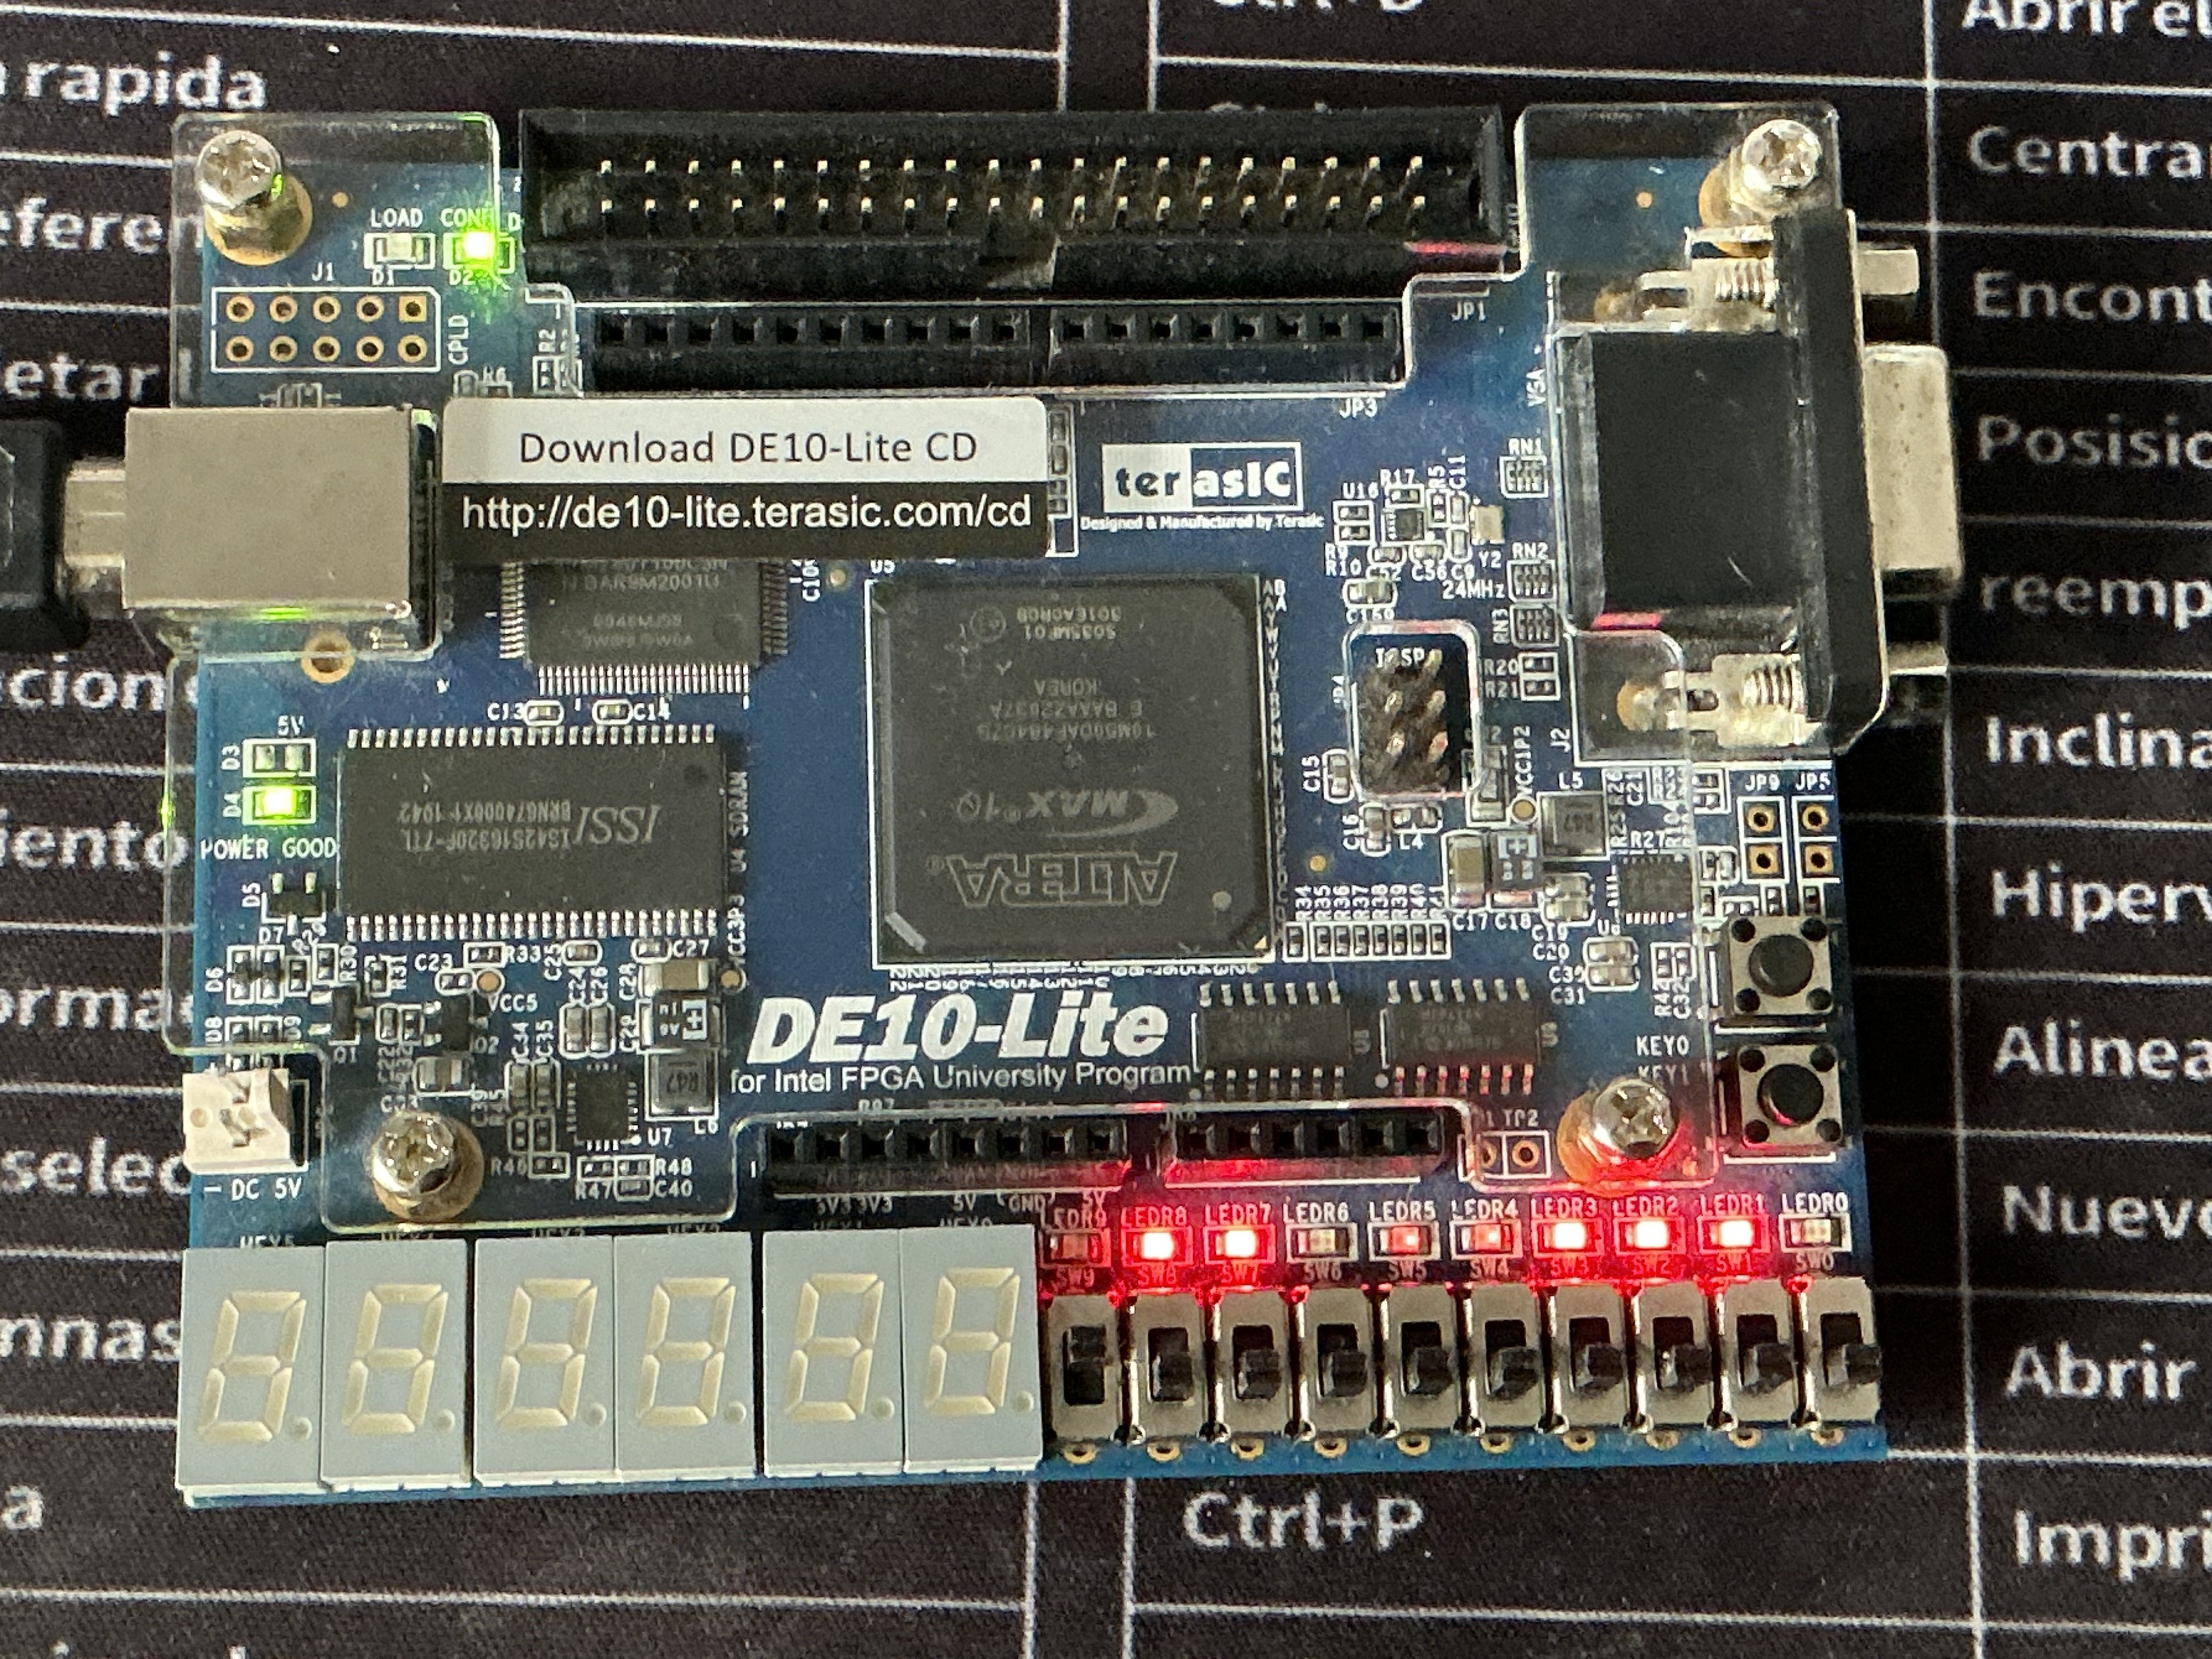
\includegraphics[width=\linewidth]{est06.jpg}\caption{$E_6$}\end{subfigure}\hfill
\begin{subfigure}[b]{0.19\linewidth}\centering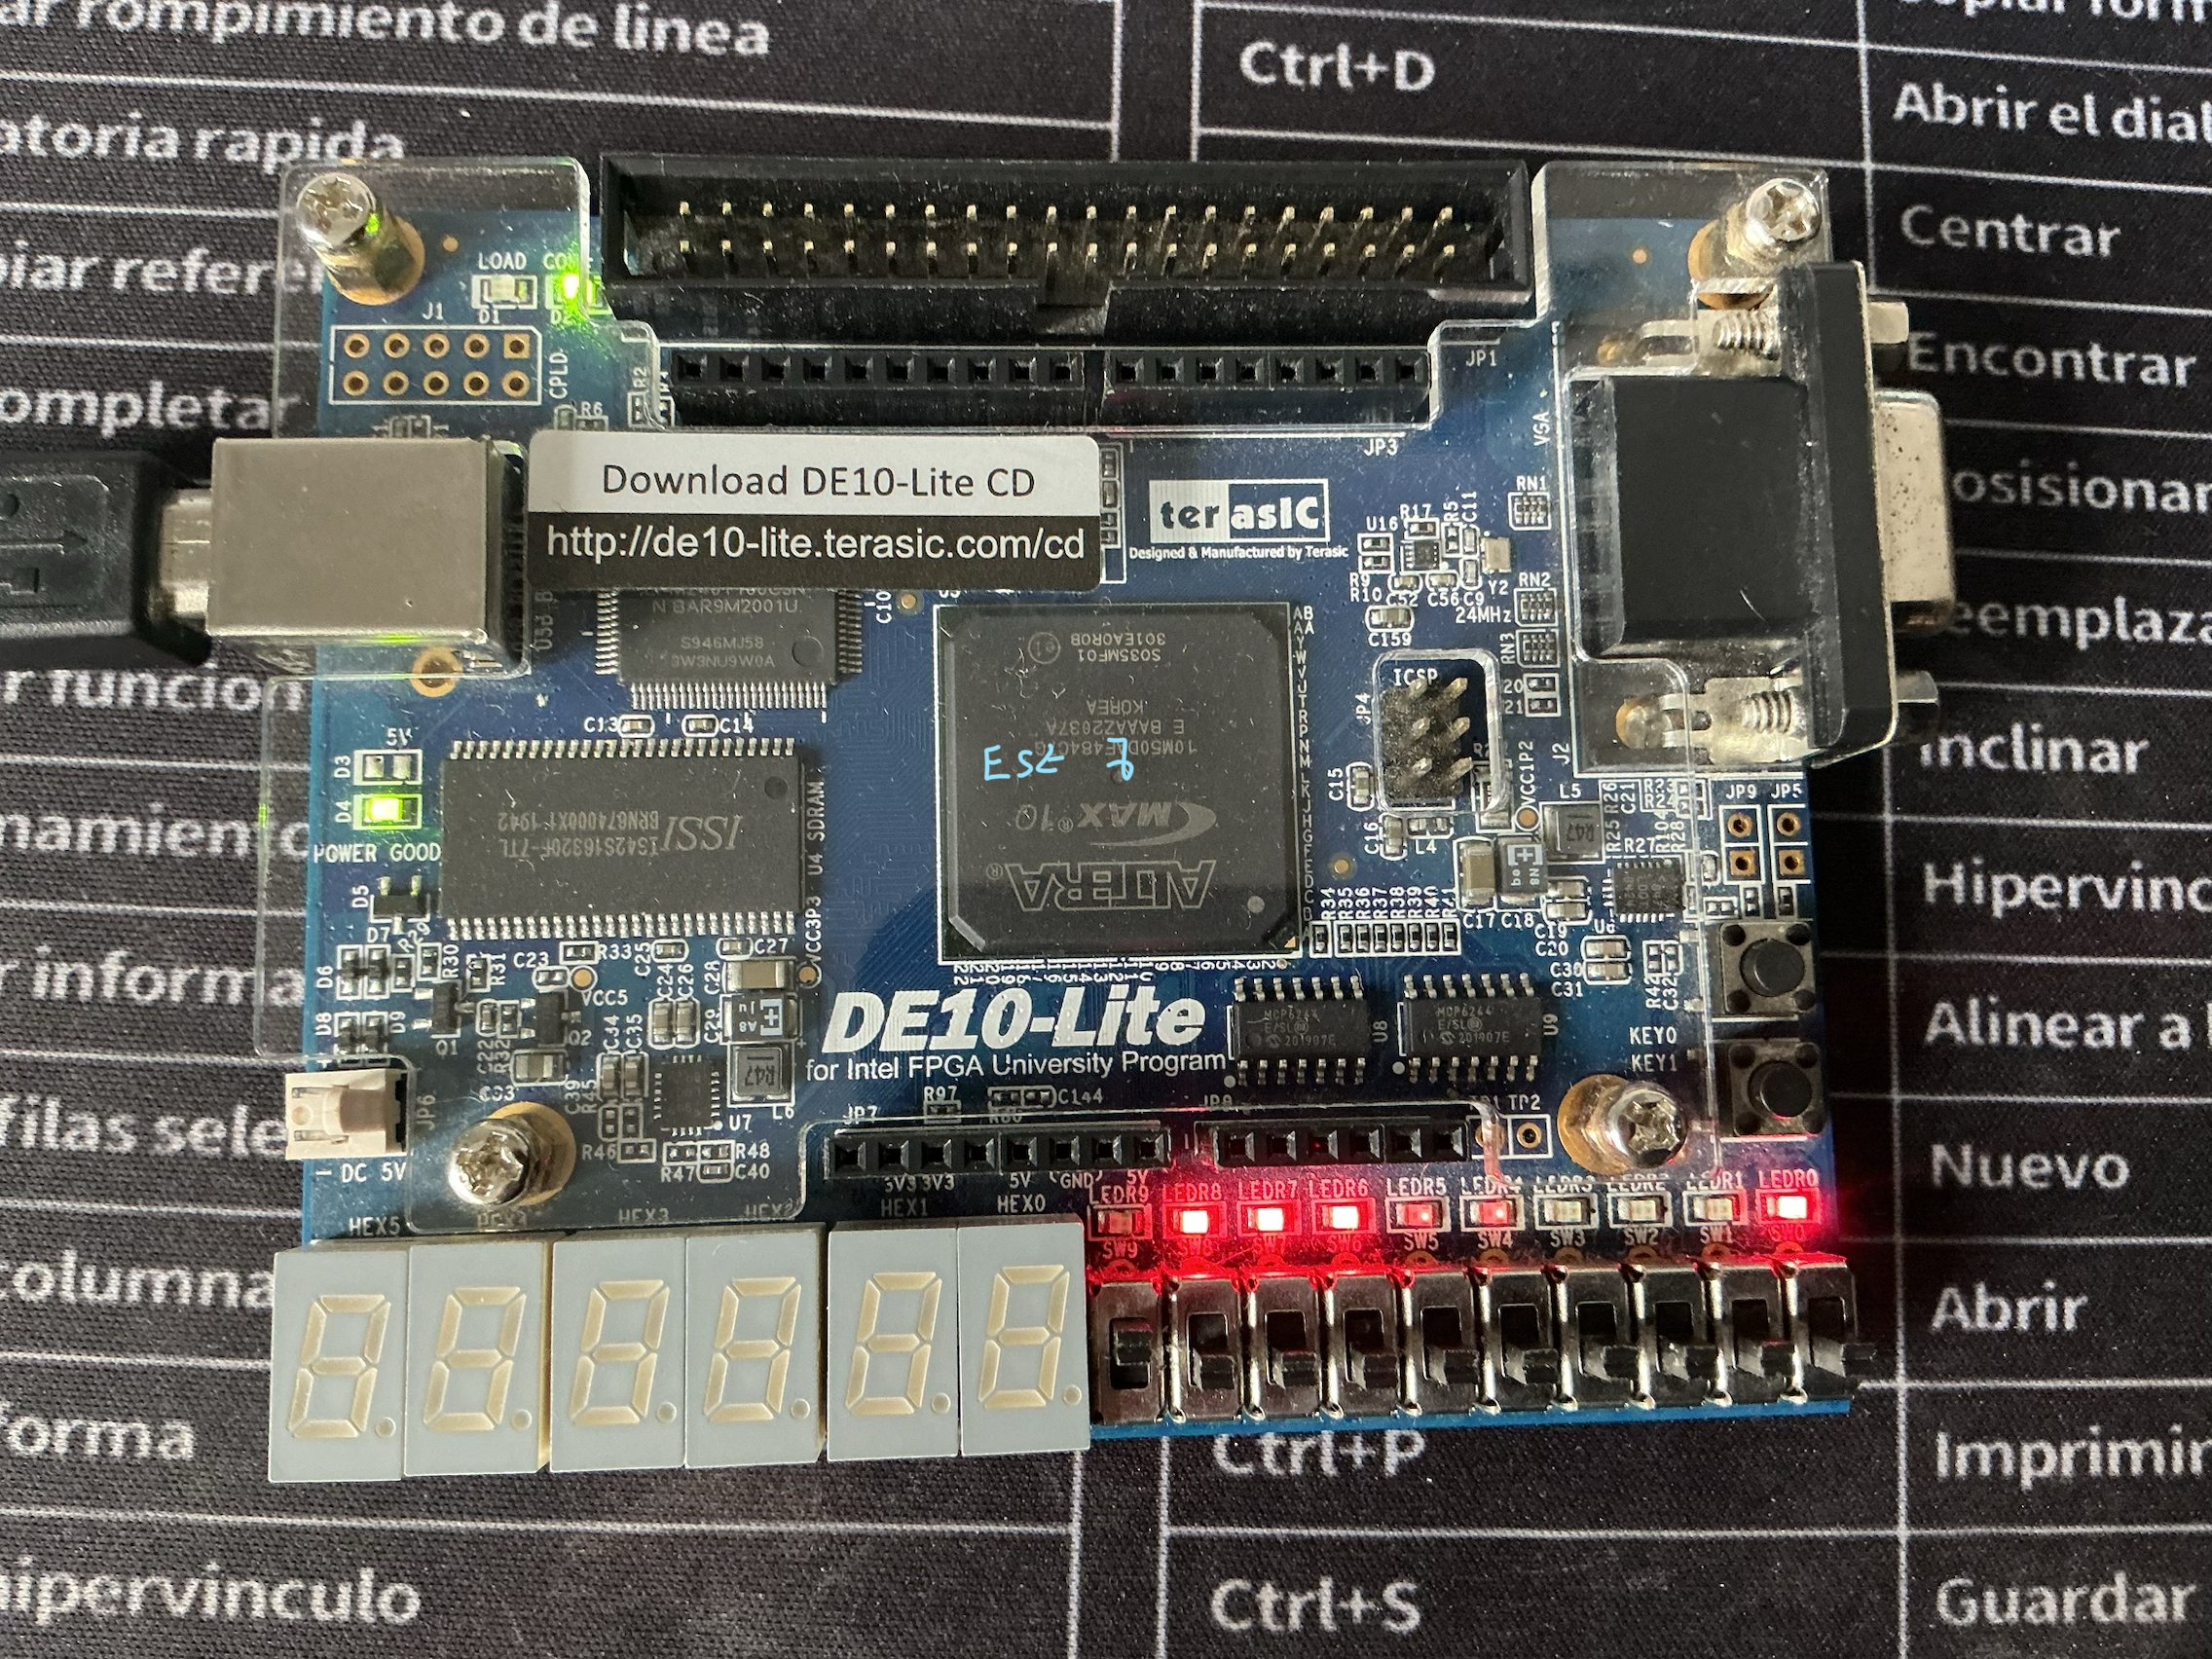
\includegraphics[width=\linewidth]{est07.jpg}\caption{$E_7$}\end{subfigure}\hfill
\begin{subfigure}[b]{0.19\linewidth}\centering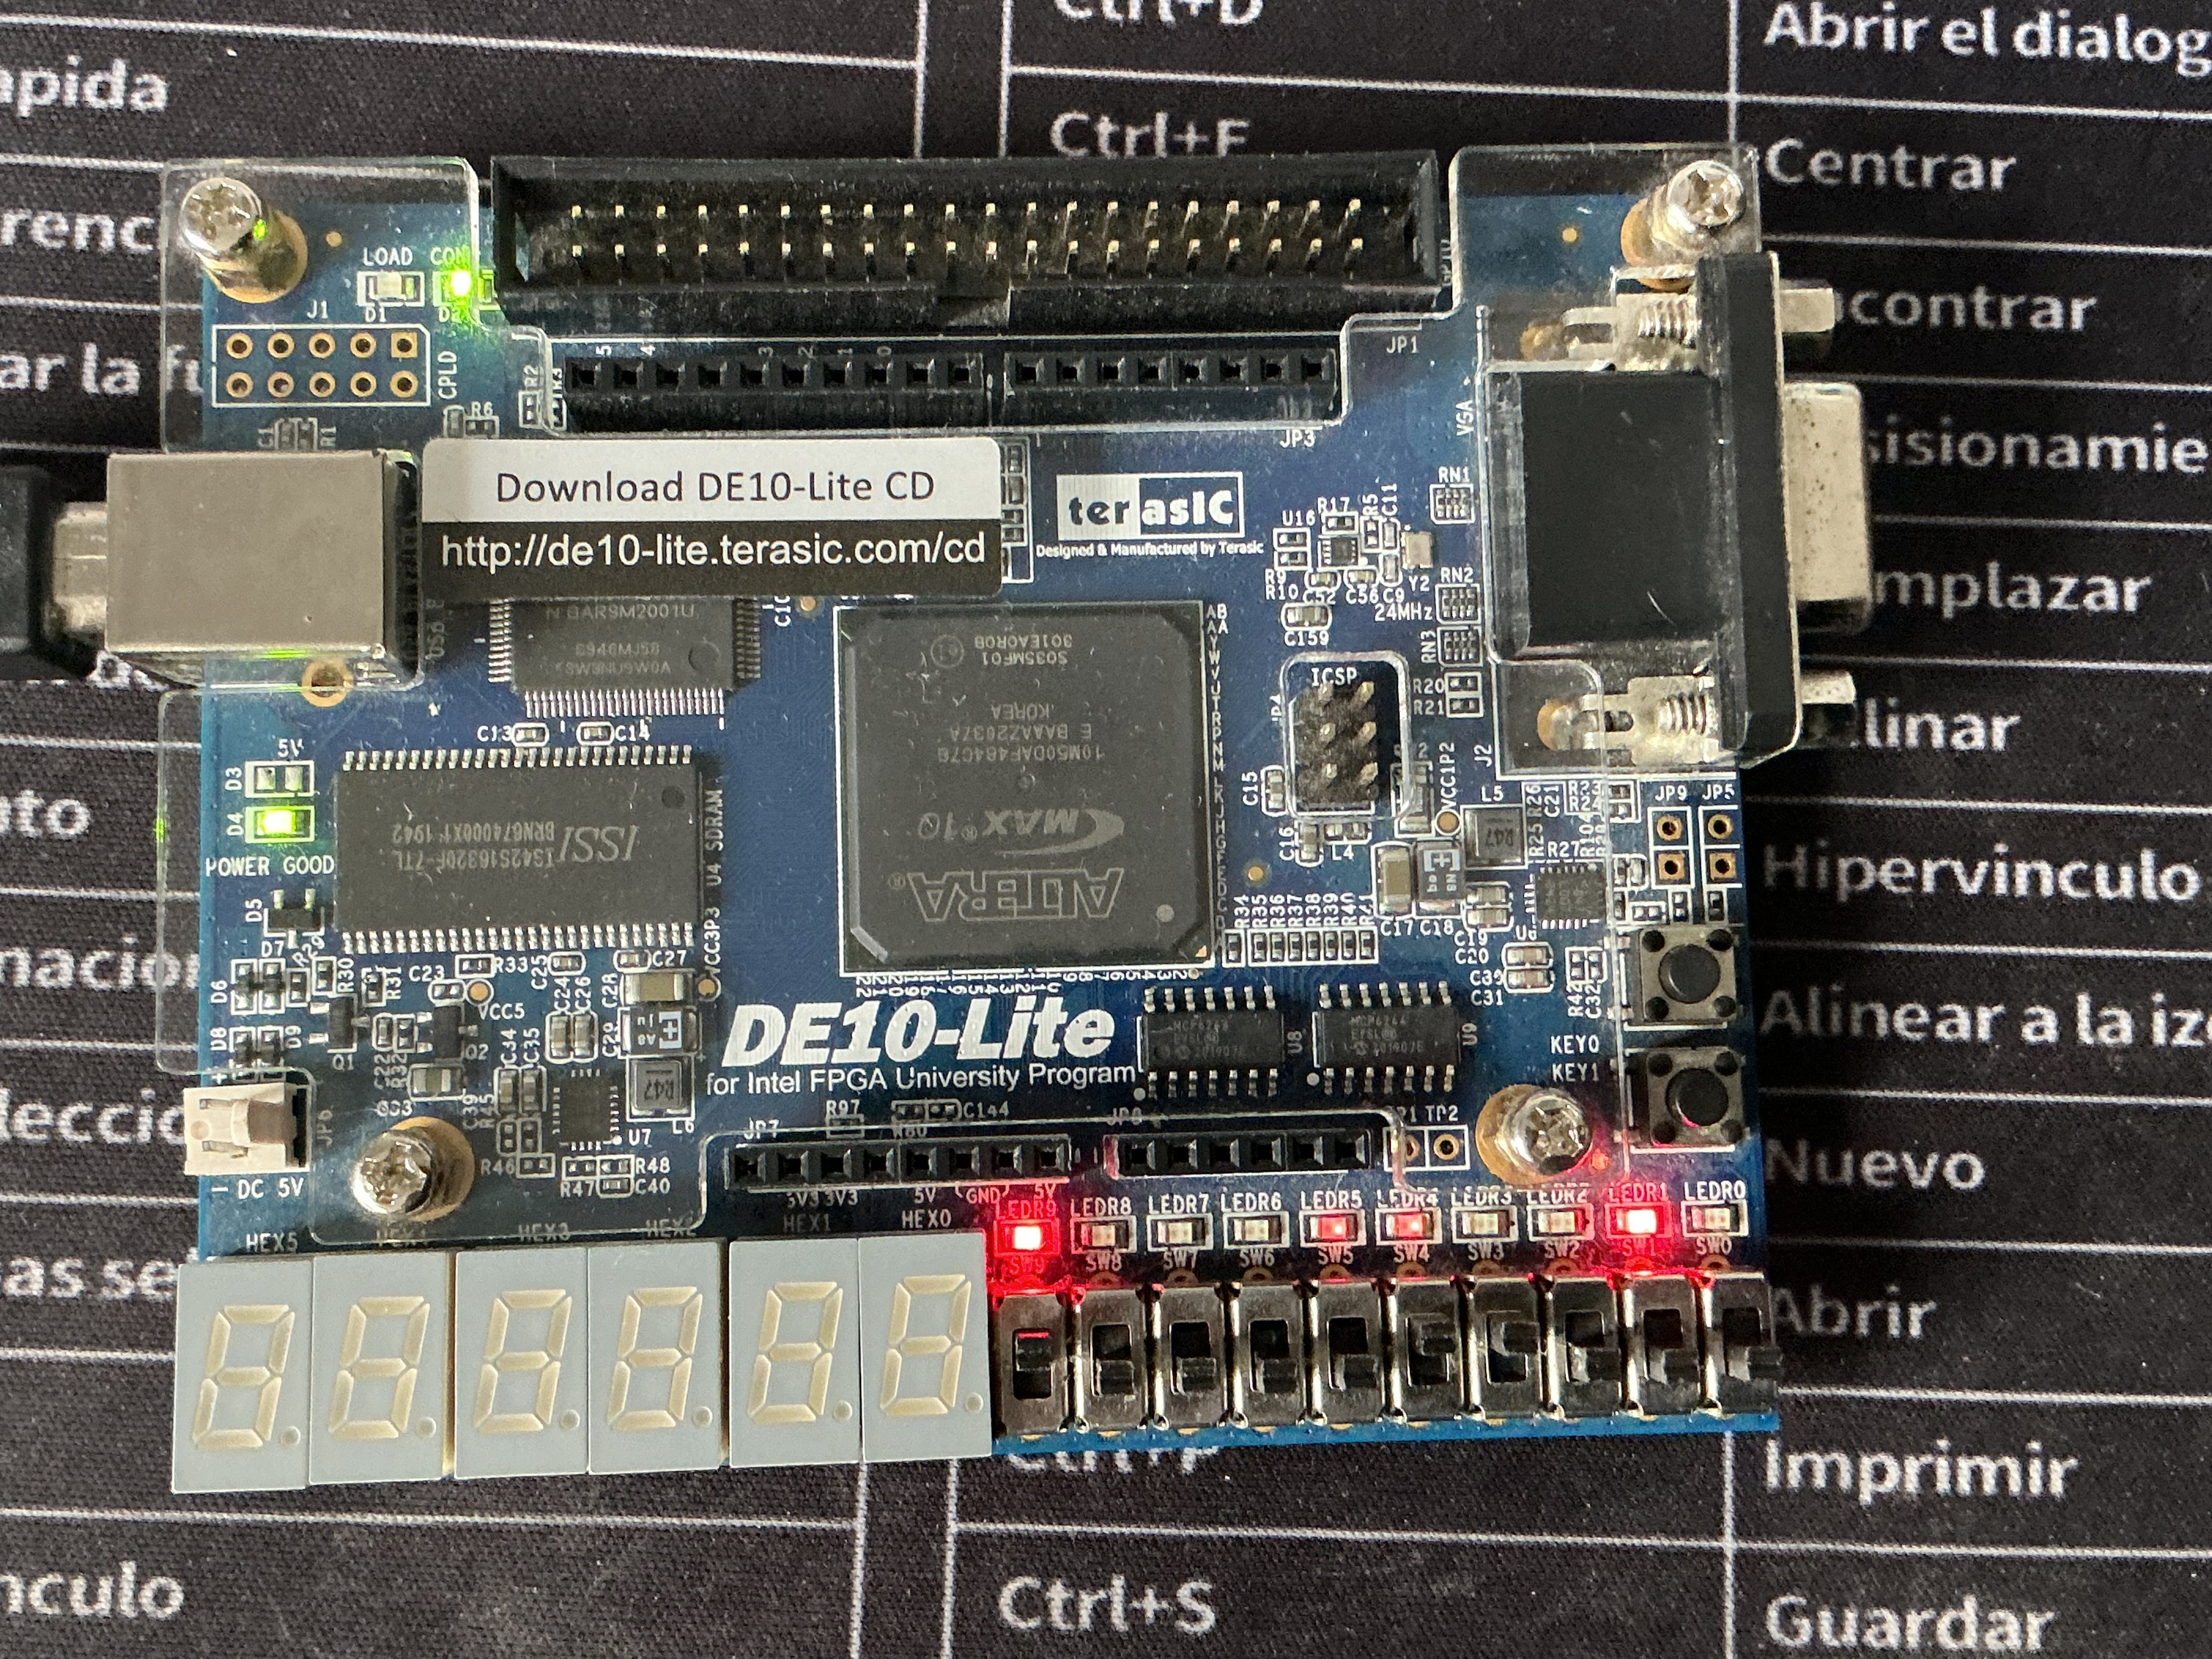
\includegraphics[width=\linewidth]{est08.jpg}\caption{$E_8$}\end{subfigure}\hfill
\begin{subfigure}[b]{0.19\linewidth}\centering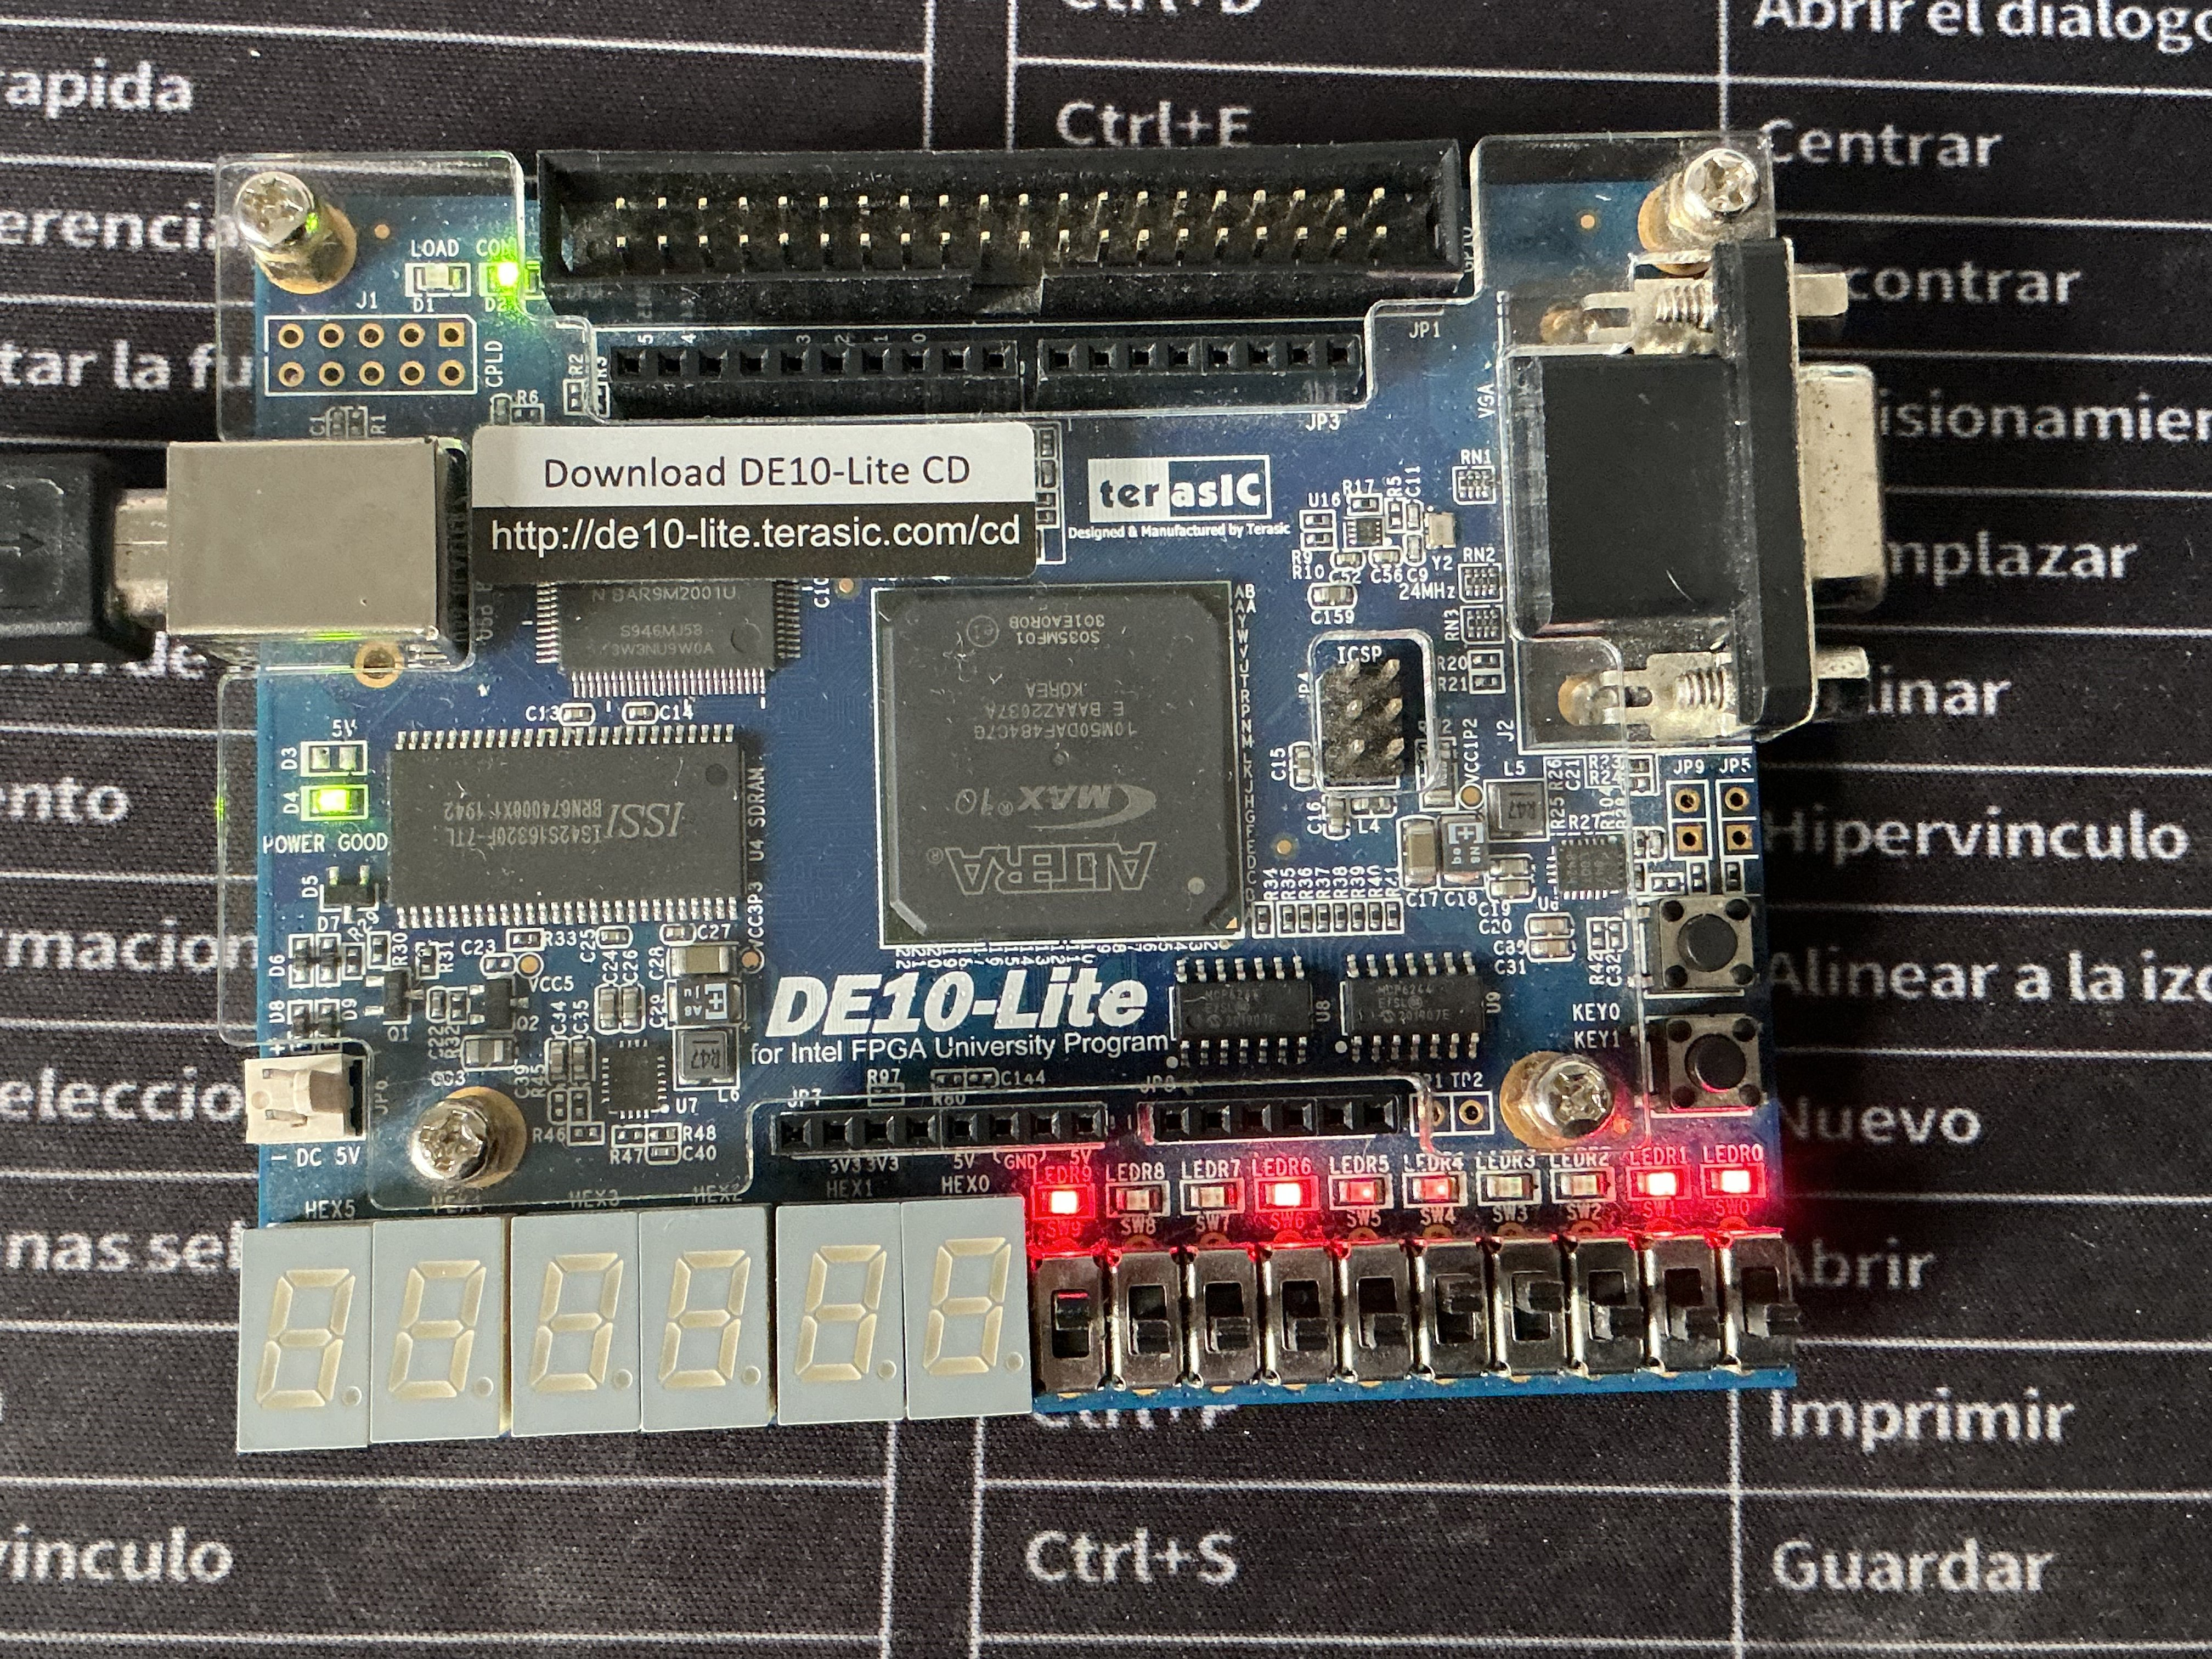
\includegraphics[width=\linewidth]{est09.jpg}\caption{$E_9$}\end{subfigure}
\caption{Comprobación física de los estados $E_5$ a $E_9$.}
\label{fig:fpga-5-9}
\end{figure}

\begin{figure}[H]
\centering
\begin{subfigure}[b]{0.19\linewidth}\centering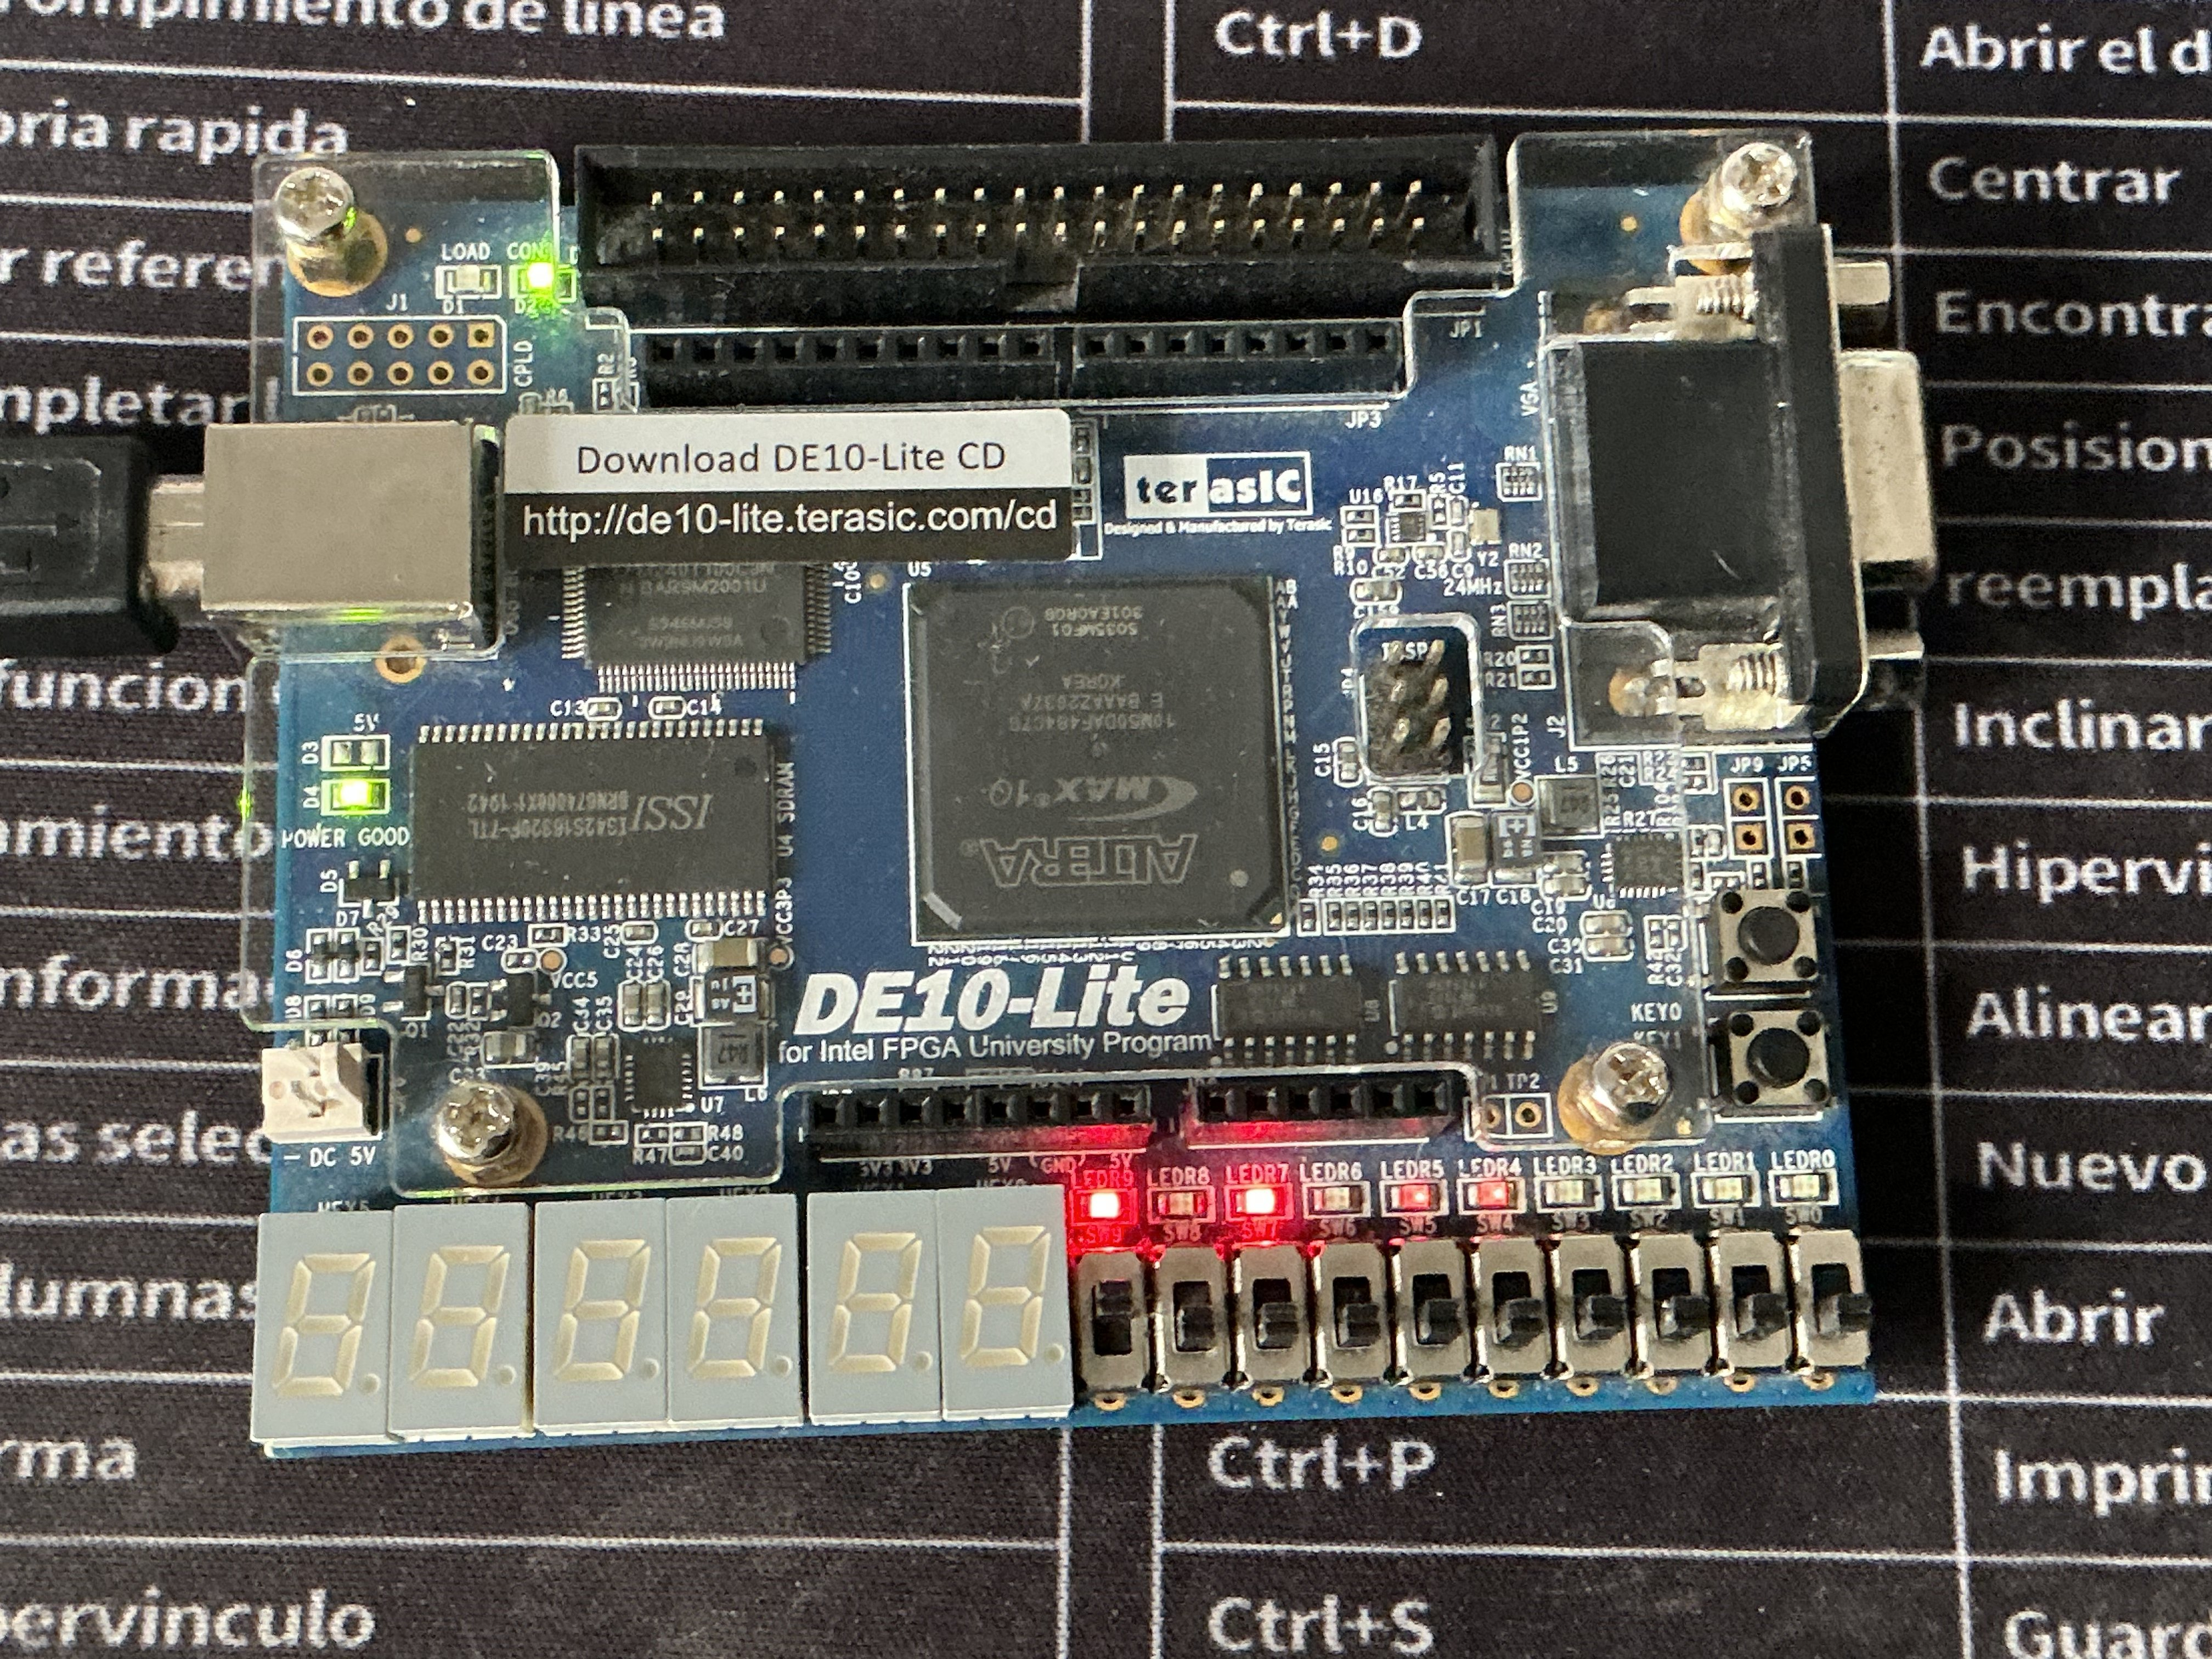
\includegraphics[width=\linewidth]{est10.jpg}\caption{$E_{10}$}\end{subfigure}\hfill
\begin{subfigure}[b]{0.19\linewidth}\centering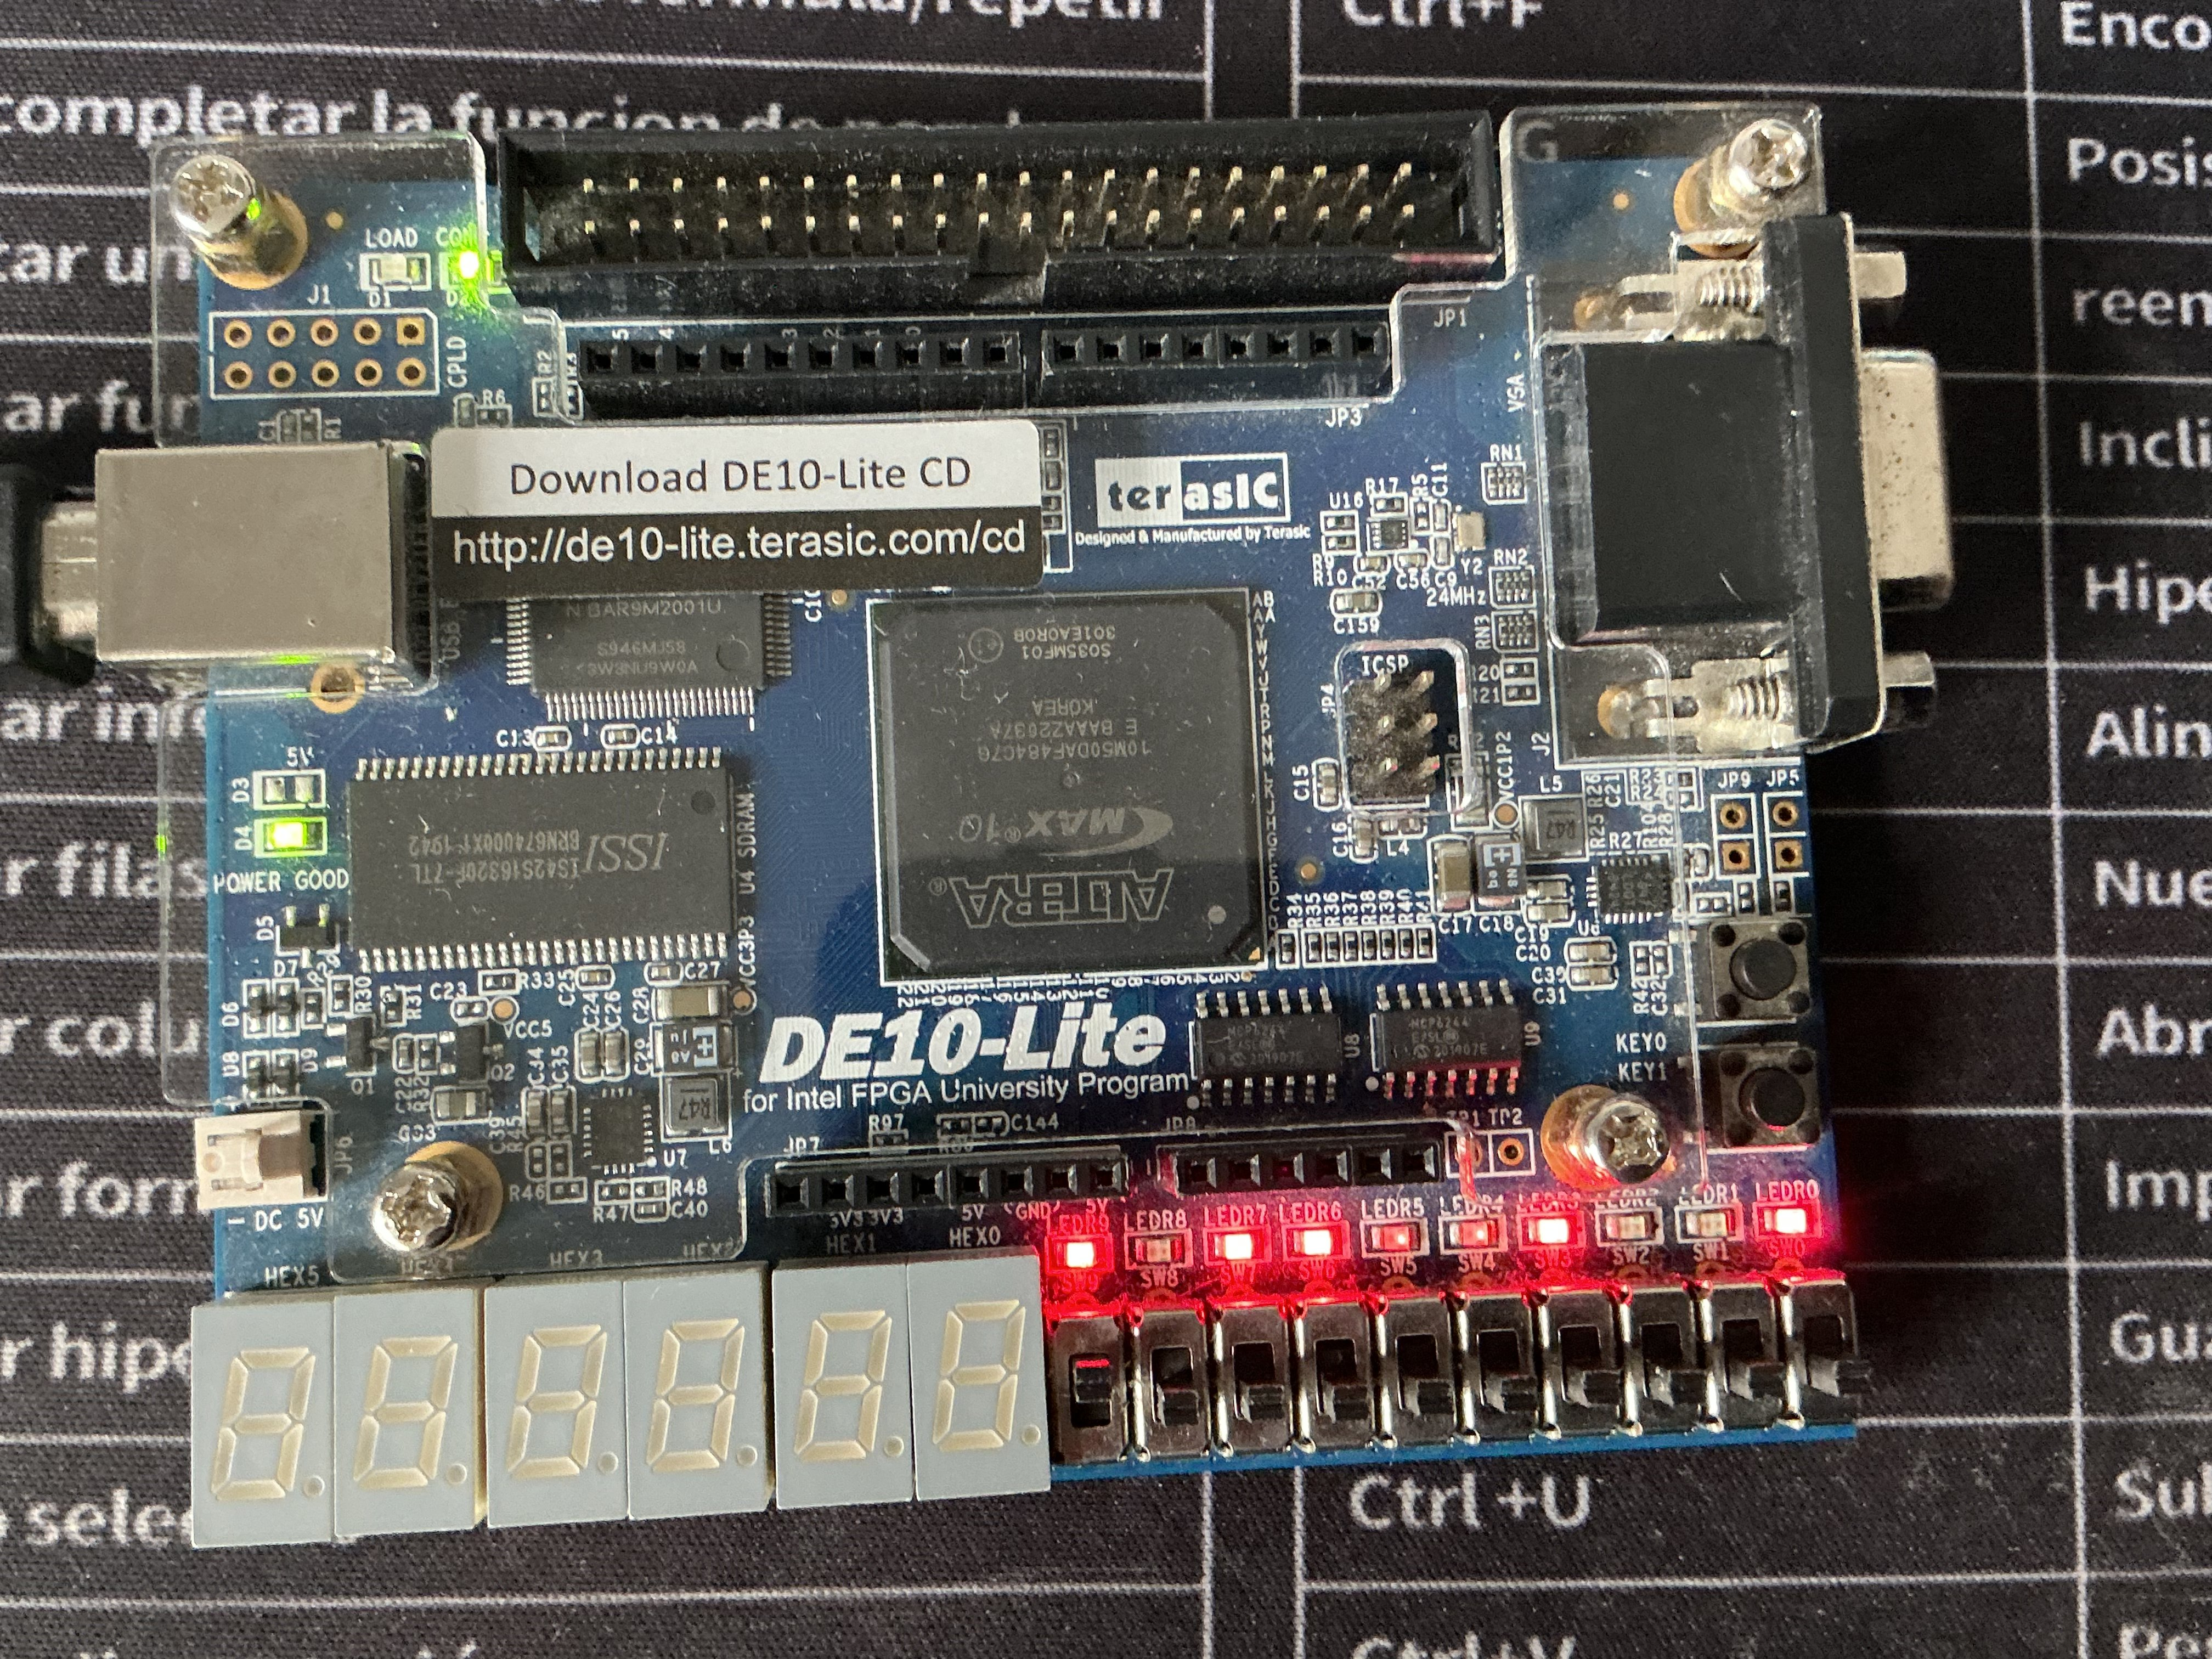
\includegraphics[width=\linewidth]{est11.jpg}\caption{$E_{11}$}\end{subfigure}\hfill
\begin{subfigure}[b]{0.19\linewidth}\centering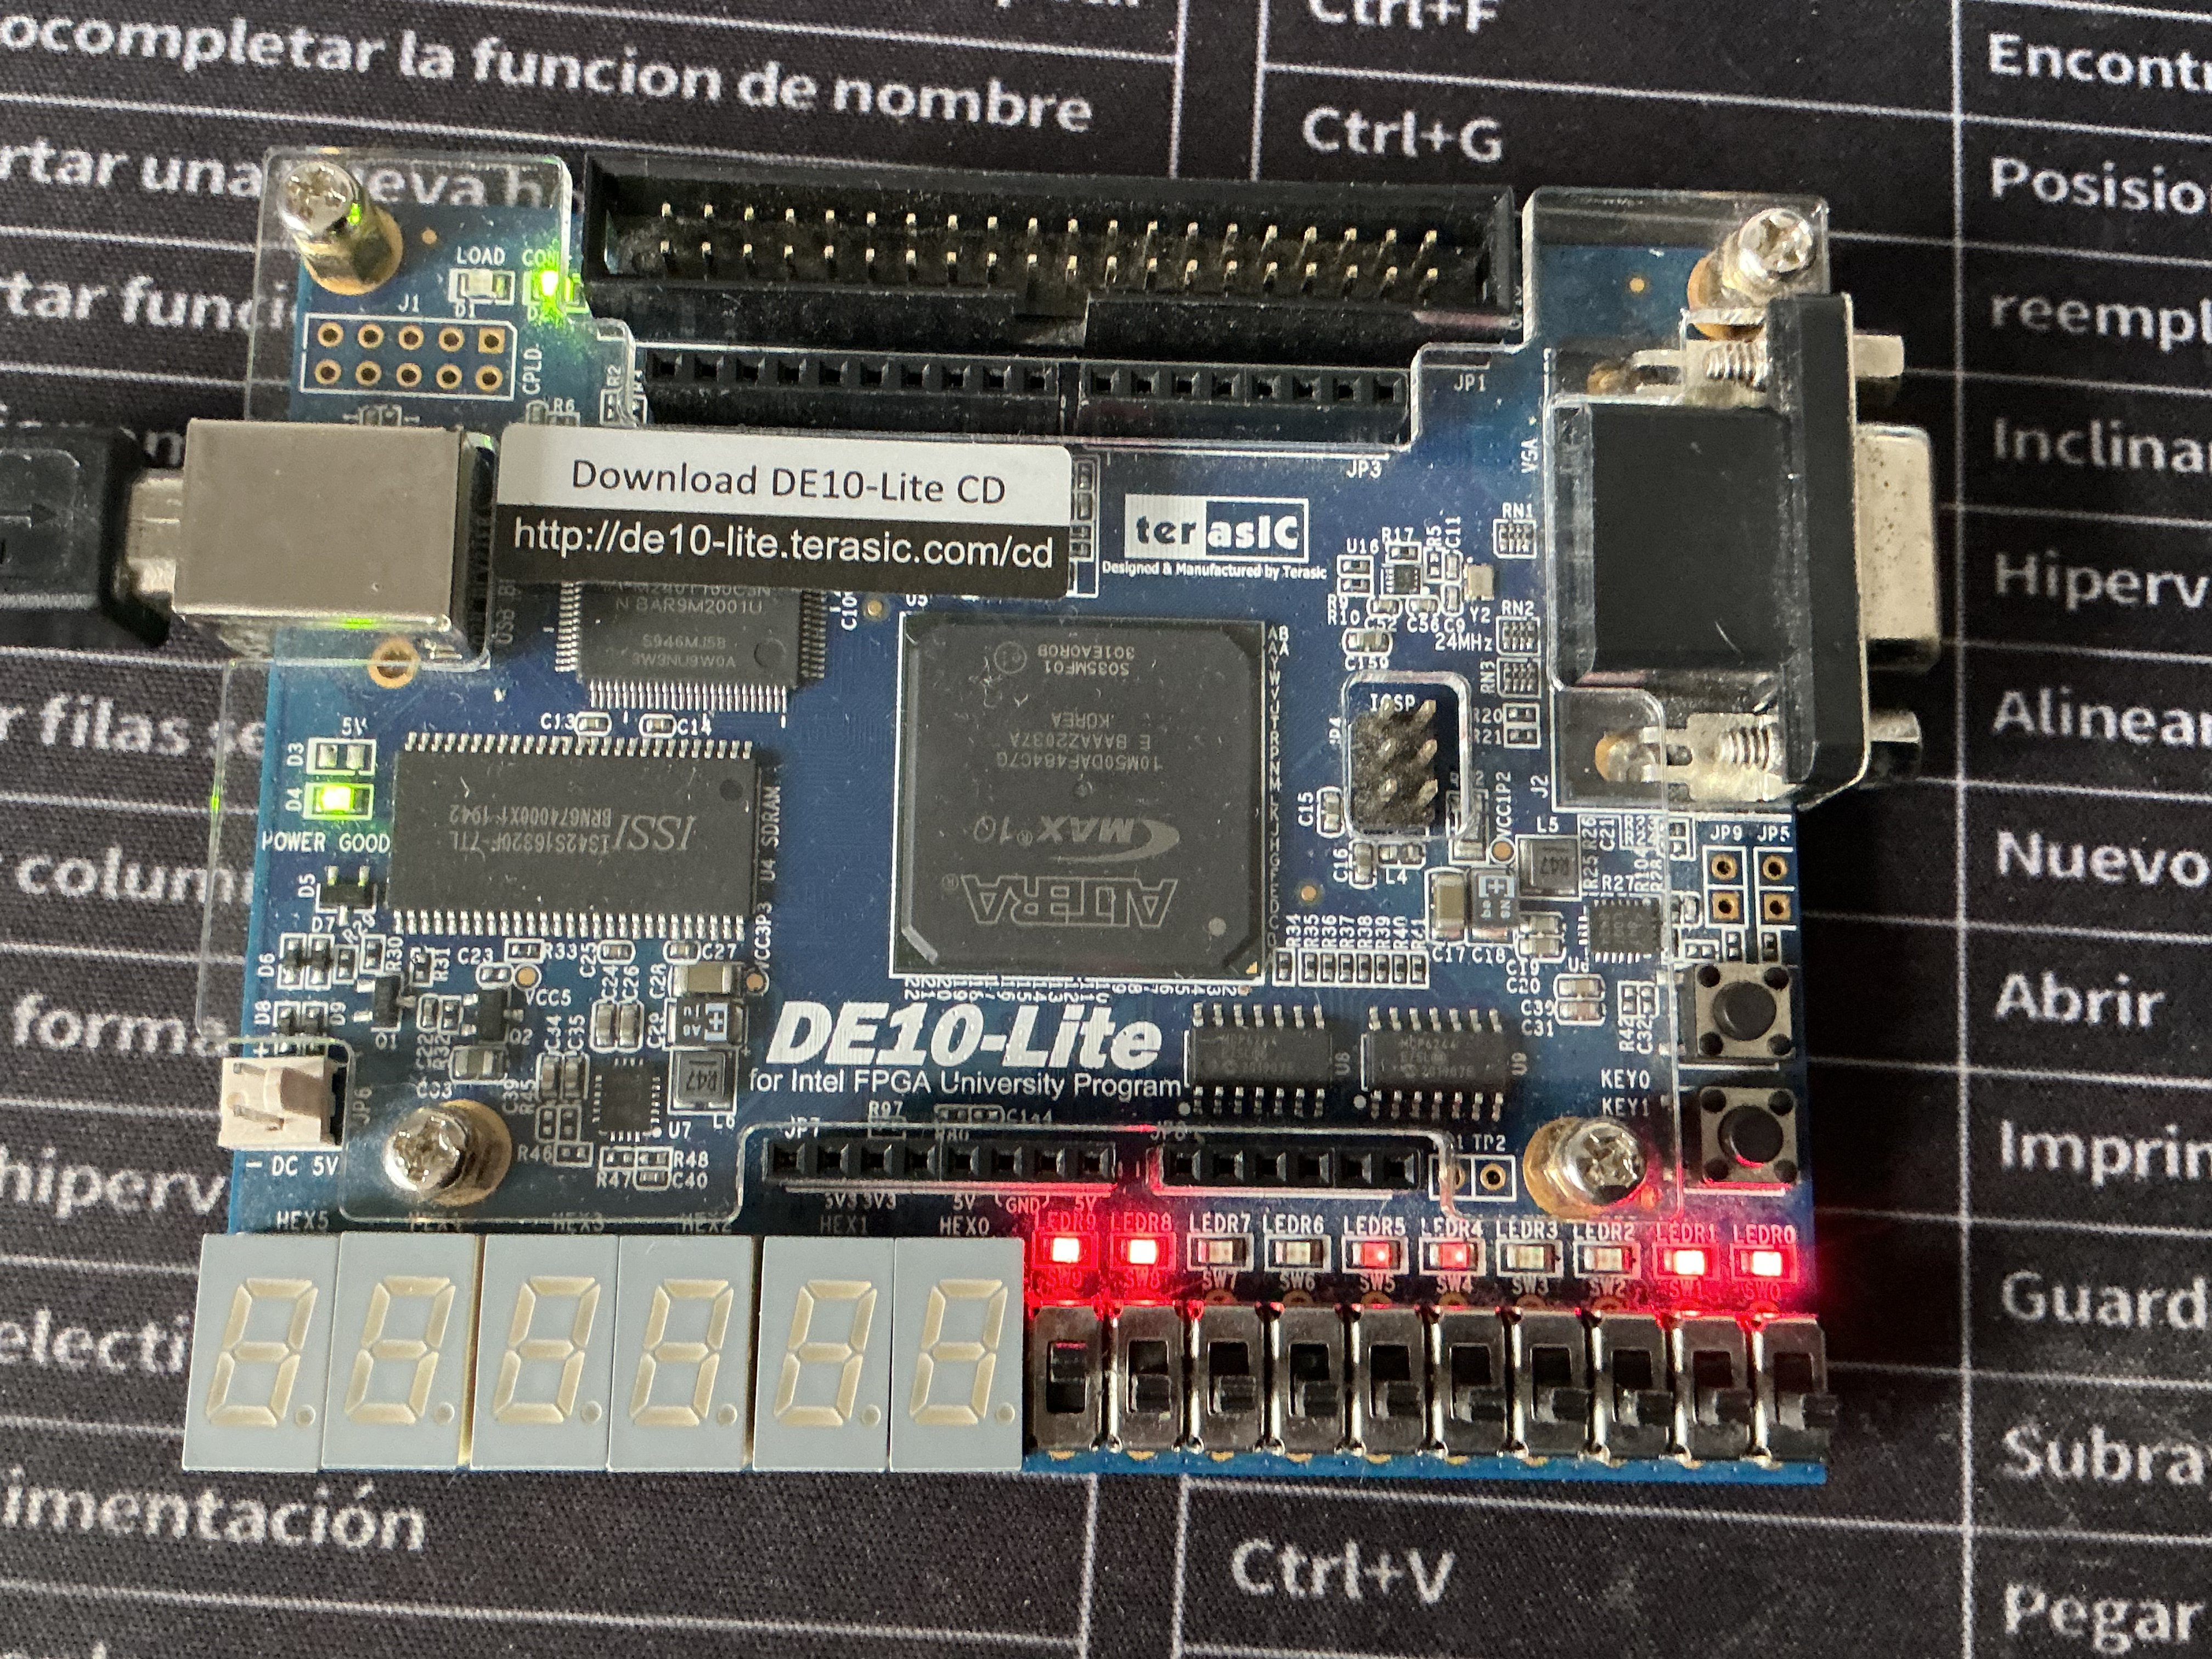
\includegraphics[width=\linewidth]{est12.jpg}\caption{$E_{12}$}\end{subfigure}\hfill
\begin{subfigure}[b]{0.19\linewidth}\centering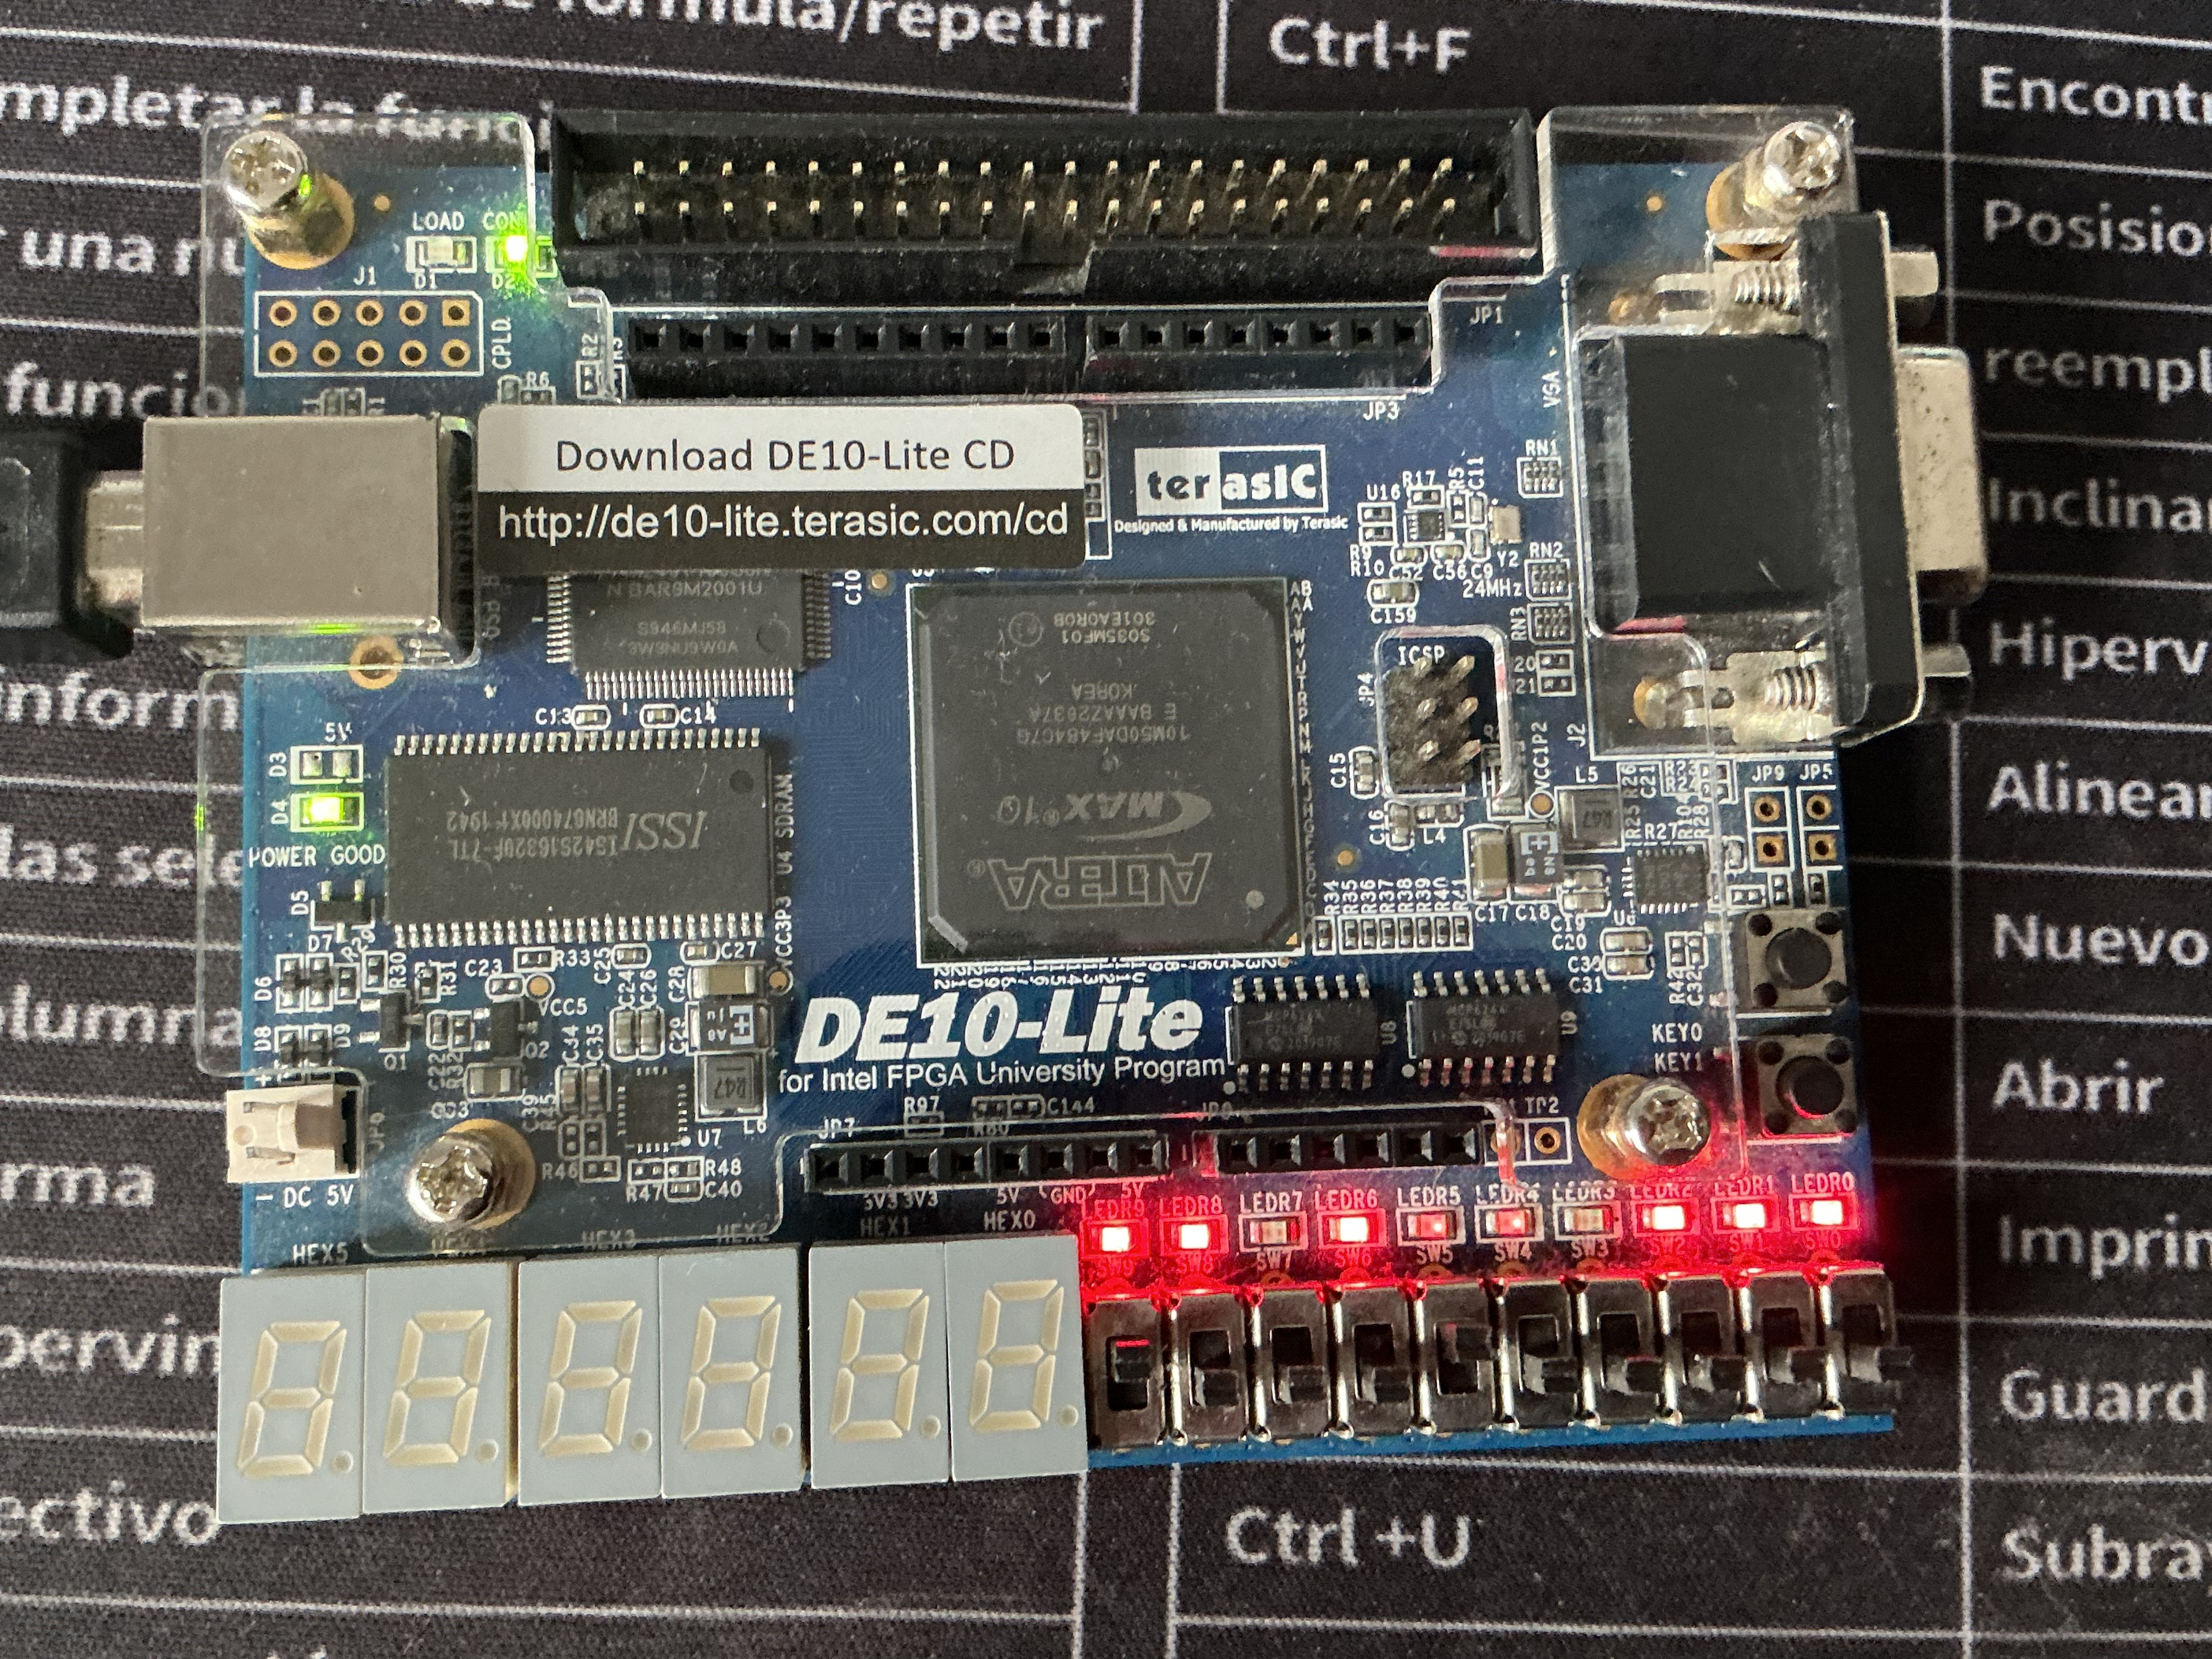
\includegraphics[width=\linewidth]{est13.jpg}\caption{$E_{13}$}\end{subfigure}\hfill
\begin{subfigure}[b]{0.19\linewidth}\centering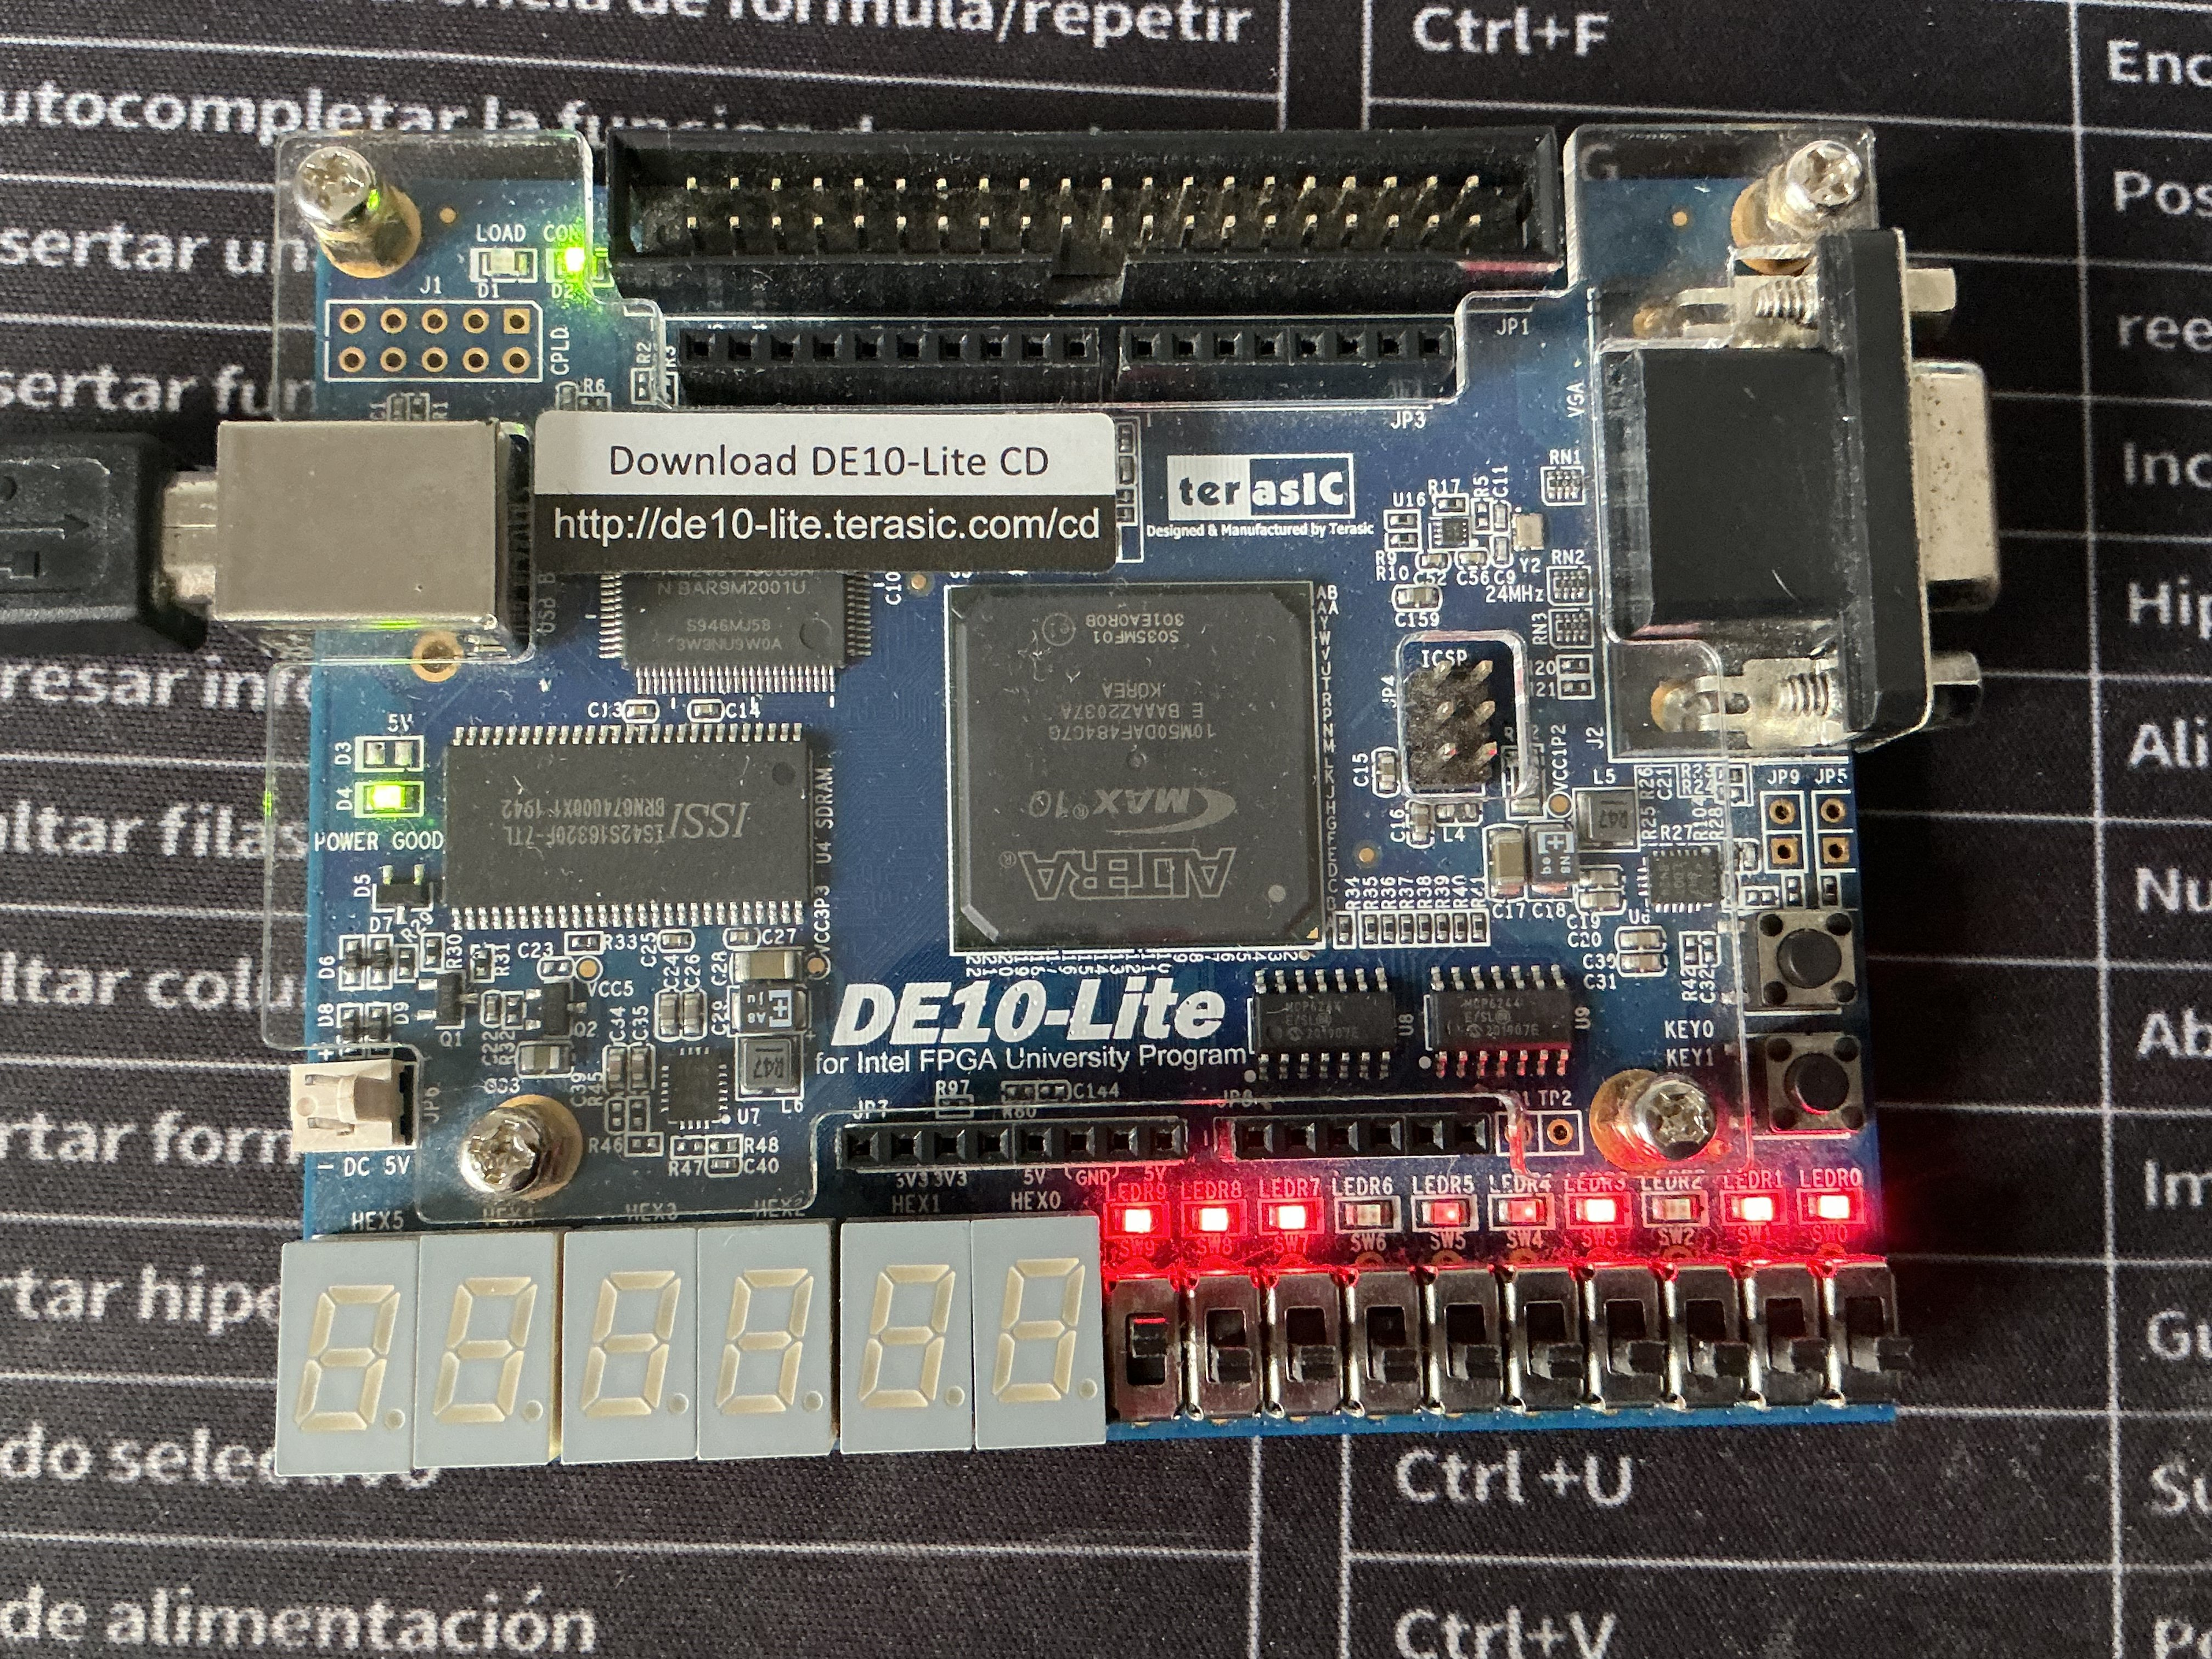
\includegraphics[width=\linewidth]{est14.jpg}\caption{$E_{14}$}\end{subfigure}
\caption{Comprobación física de los estados $E_{10}$ a $E_{14}$.}
\label{fig:fpga-10-14}
\end{figure}

\section{Conclusión}

\paragraph{Percival Ulises Espinoza Matamoros.} El desarrollo de esta práctic me permitió comprender mejor la importancia del secuenciador. Al implementar la carta ASM con interrupciones y transformaciones, se observó que el secuenciador es un componente fundamental para el control del sistema, ya que genera la secuencia de microinstrucciones y selecciona la siguiente microdirección de acuerdo con las condiciones y el estado presente. A demás la implementación propuesta ara la transformación e interrupción permite poder implementar de manera sencilla y clara la carta ASM, ya que se puede cambiar el estado de transformación o interrupción sin necesidad de modificar el secuenciador.

\paragraph{Oscar Iván Montiel Juárez.} El desarrollo permitió relacionar la carta ASM con una implementación real en VHDL. La ROM de $16 \times 13$ bits concentra la secuencia de control, mientras que el contador de microprograma y los multiplexores seleccionan la dirección siguiente. La simulación y la tarjeta mostraron que los saltos condicionados, las transformaciones y las interrupciones se realizan de acuerdo con el estado presente.

\paragraph{Amy Valentina Veraza García.} La práctica reforzó la importancia de dividir una microinstrucción en campos independientes. Al observar los LEDs se pudo comprobar que las salidas de cada estado se obtienen directamente de la ROM y que el botón permite avanzar de forma controlada para verificar la secuencia definida en la carta ASM.

\end{document}
